\chapter{Conjuntos de corte y ciclos}

\lettrine[lines=5] {\initfamily \selectfont E} {l concepto} central de este capítulo es el de \textit{subgráfica generadora}. Además, abordaremos tres clases especiales de subgráficas: los \textit{conjuntos de corte}, las \textit{subgráficas pares} y los \textit{árboles generadores}. Recuérdese que, si $G$ es una gráfica, una subgráfica de $G$, digamos $H$, es \textit{generadora} si y sólo si $V(H)=V(G)$. Igualmente, vimos en el capítulo anterior que $G[S]$ es una \textit{subgráfica inducida por aristas} si y sólo si $E(G[S]) = S\subseteq E(G)$ y su conjunto de vértices queda determinado por los extremos de las aristas en $S$; y $G[S]$ es una \textit{subgráfica generadora inducida por aristas} si y sólo si $V(G[S]) = V(G)$ y $E(G[S]) = S\subseteq E(G)$. A lo largo de este trabajo, el símbolo ``$G[S]$" denotará a una subgráfica generadora inducida por el conjunto aristas $S$. 



\section{Conjuntos de corte de $G$}

Supongamos que $G$ es una gráfica cualquiera. Tomando $X$ y $Y$ dos subconjuntos de vértices de $G$, denotaremos por $E[X,Y]$ al subconjunto de aristas de $G$ que tienen un extremo en $X$ y otro en $Y$. Si $X = Y$, sólo escribiremos $E[X]$. Si sucediera que $Y$ es el complemento de $X$ respecto a $V$, es decir, que $Y=V \setminus X$, entonces al conjunto $E[X, V \setminus X]$ se le llamará \textit{conjunto de corte de $G$ asociado a $X$} \index{Conjunto de corte! de $G$ asociado a $X$} y será escrito como $\partial(X)$. Si $H$ es una subgráfica de $G$ y $X \subseteq V(H)$, entonces $\partial_{H}(X):= E[X, V(H)\setminus X]$ denota al \textit{conjunto de corte asociado a $X$ relativo a $H$}  \index{Conjunto de corte! asociado a $X$ respecto a $H$}. Los conjuntos de cortes relativos serán de utilidad cuando se hable de gráficas inconexas (ver ejemplo \ref{ejem:relativos}).

Por comodidad, en lo sucesivo escribiremos $\overline{X}$ en lugar de $V \setminus X$. Así, $\partial(X) = E[X,\overline{X}]$. Es sencillo observar que $\partial(X) = \partial(\overline{X})$ pues, por definición, $E[X,\overline{X}] = E[\overline{X},X]$. En particular, $\partial(V)=\partial(\emptyset) = \emptyset$ (y, por lo tanto, $\emptyset$ es un conjunto de corte). También puede deducirse que, para cada  $v \in V$, $\partial(\{v\})$ es el conjunto de todas las aristas que inciden en $v$, excluyendo sus lazos.  A veces escribimos $\partial(v)$ en lugar de $\partial(\{v\})$.

$G\Big[\partial(X)\Big]$ denotará a la subgráfica generadora de $G$ inducida por el conjunto aristas $\partial(X)$. Tal subgráfica también es llamada \index{Conjunto de corte! como subgráfica generadora inducida por aristas}\textit{conjunto de corte}. Aunque lo anterior es un abuso de notación, algunos autores utilizan el mismo símbolo ``$\partial(X)$"\:\!\! para referirse a ambos conceptos: el conjunto de corte y la subgráfica generadora inducida por el conjunto de corte. Para evitar confusiones, en este trabajo preferimos no emplear este abuso de notación.


\begin{ejem} \label{ejem:cjtosdecorte}
Consideremos la gráfica del inciso $(a)$ de la figura \ref{fig:cjtosdecorte}. En $(b)$ representamos el conjunto de aristas $E[A,B] = \{b,c,f,g\}$, con $A=\{u_{1}, u_{2}, u_{3}\}$ y $B=\{u_{3},u_{4}\}$. En $(c)$ tomamos $X =\{u_{1},u_{5}\}$, y verificamos que $\partial(X) = \{a,f,g,d\}$.
\begin{figure}[H]
    \centering
    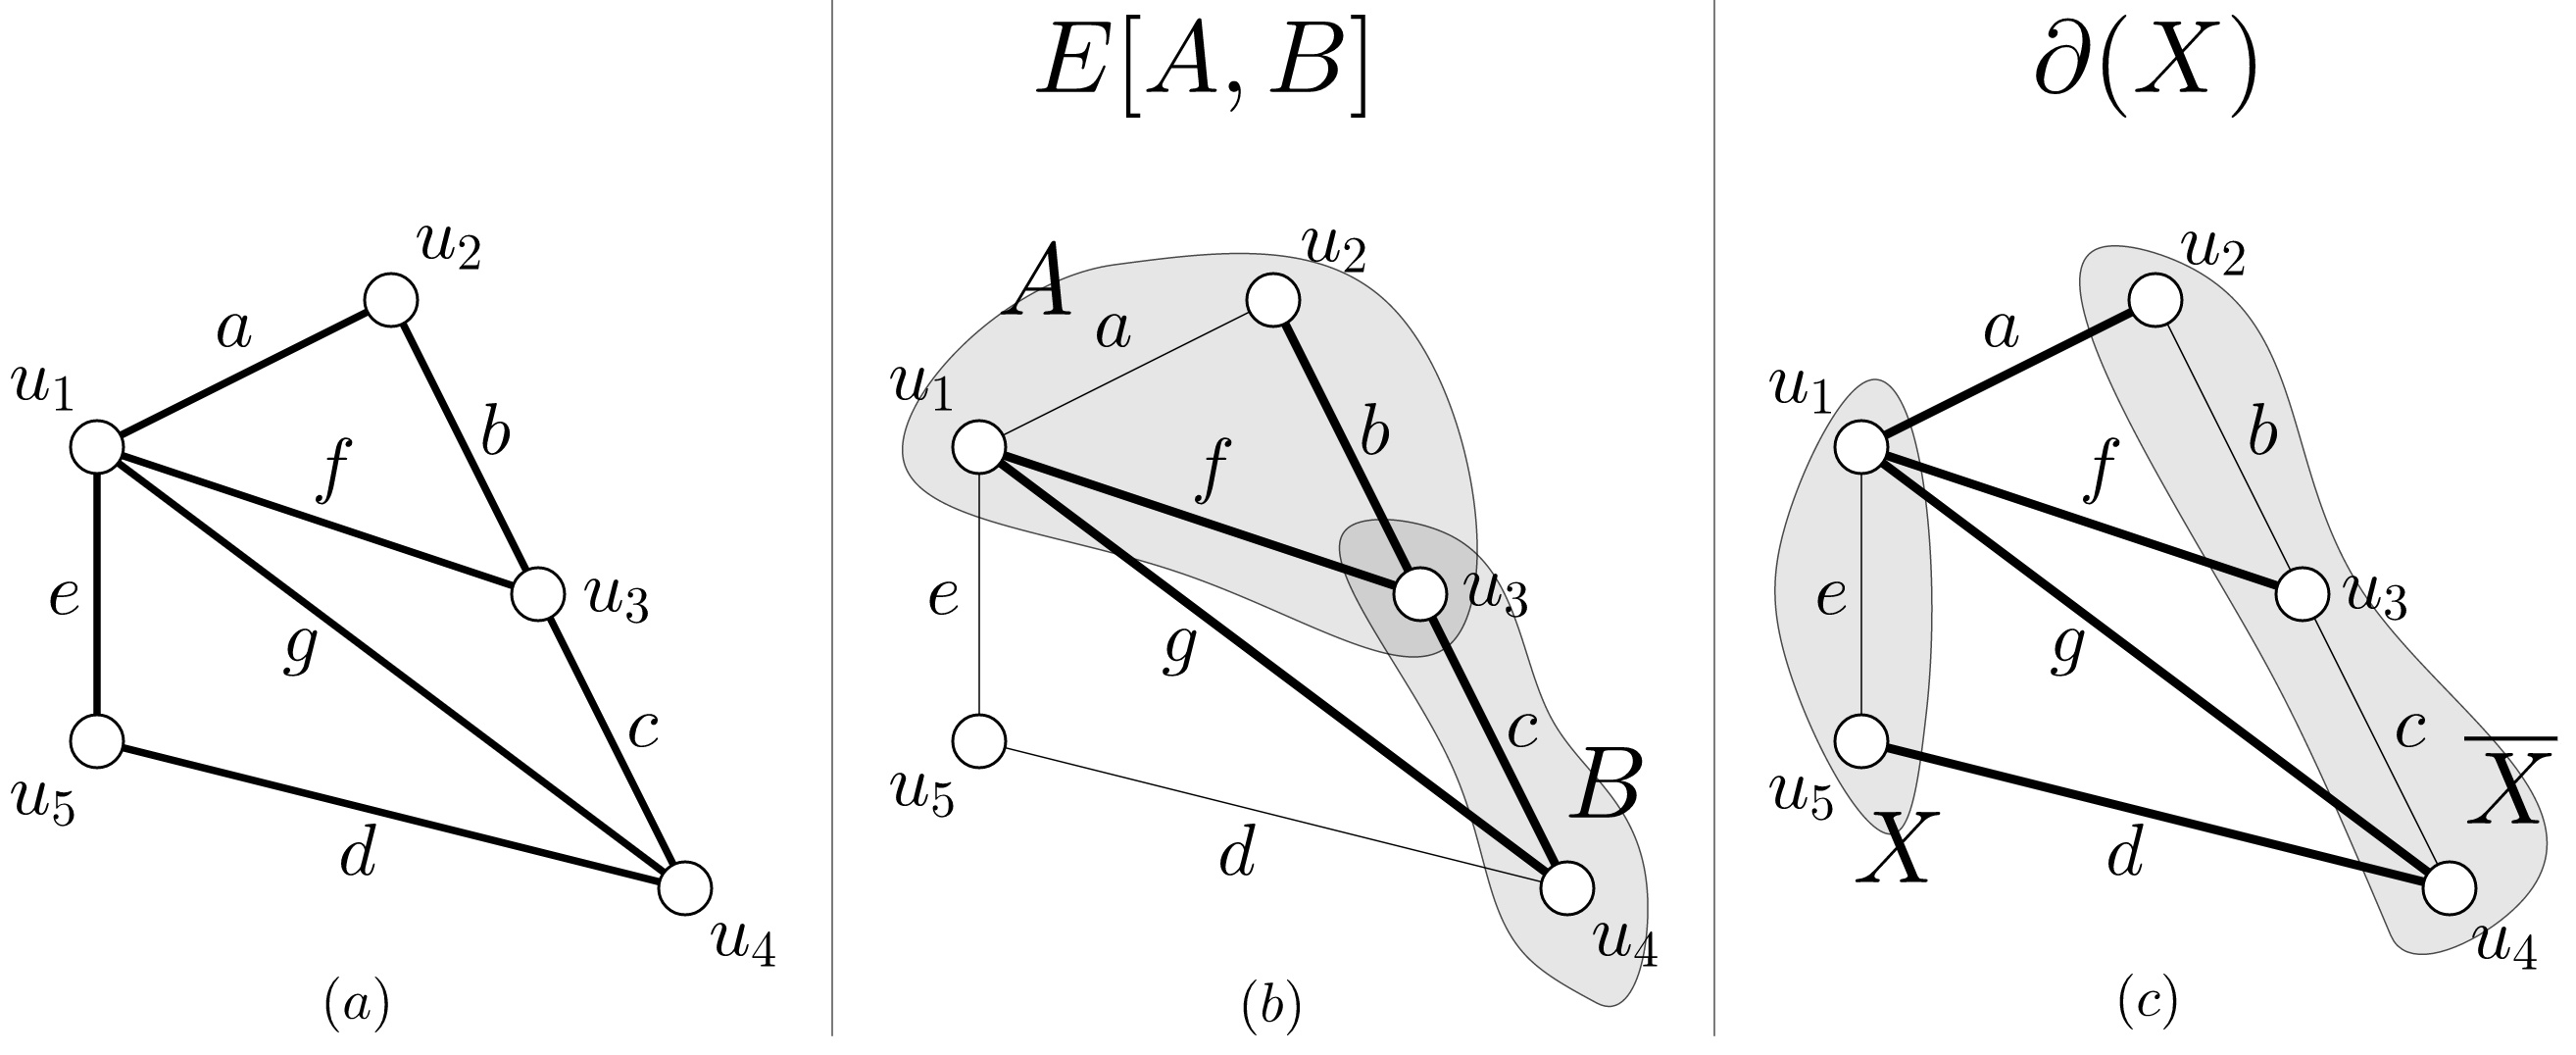
\includegraphics[scale=0.24]{img/imgchapter2/cjtosdecorte.jpg}
    \caption{}
    \label{fig:cjtosdecorte}
\end{figure}

\hfill $\blacklozenge$
\end{ejem}

\begin{ejem}\label{ejem:relativos}
\begin{figure}[H]
\vspace{-2.1cm}
    \centering
    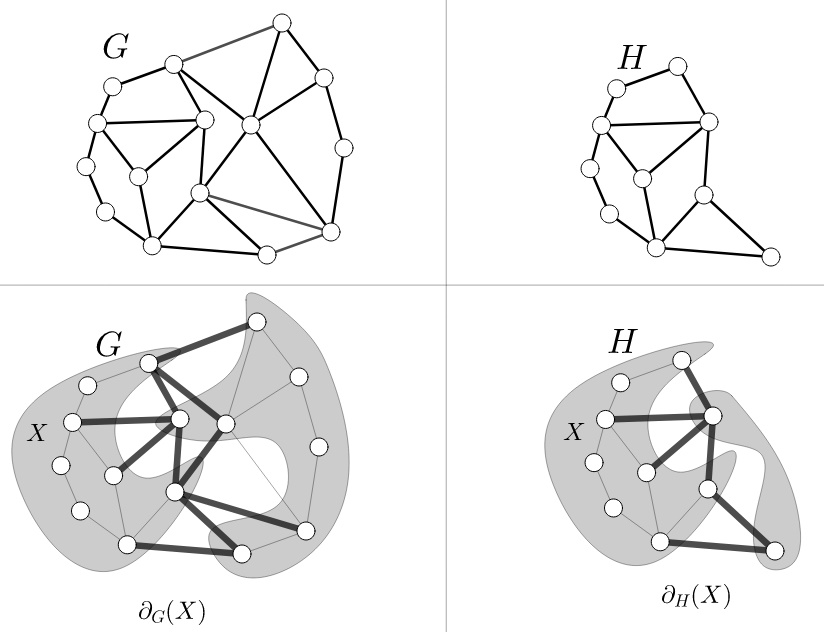
\includegraphics[scale=0.6]{img/imgchapter2/cortesrelativos.jpg}
    \caption{}
    \label{fig:corterelativo}
\end{figure}
En la figura \ref{fig:corterelativo}, $H$ es una subgráfica de $G$ y representamos el conjunto de corte $\partial(X)$ y el corte relativo a $\partial_{H}(X)$. Nótese que, a pesar de tener en común el conjunto $X$, en general, $\partial(X) \neq \partial_{H}(X)$

\hfill $\blacklozenge$
\end{ejem}
Observe que la definición de conjunto de corte ayuda reformular la concepto de \textit{gráfica conexa} que dimos en el capítulo anterior (y que utilizaremos en los teoremas siguientes): \textit{una gráfica $G$ es conexa si y sólo si $\partial(X) \neq \emptyset$, para todo $X \subsetneqq V(G)$}. De hecho, suponiendo que $G$ es conexa, podemos darnos cuenta que, eliminando de $G$ las aristas que pertenecen a $\partial(X)$, la subgráfica $G\setminus \partial(X)$ será inconexa (justificando así el nombre que se le dio a $\partial(X)$). 
\begin{ejem}
Si tomamos en cuenta la gráfica del ejemplo \ref{ejem:cjtosdecorte} y hacemos $X=\{u_{1},u_{4}\}$, vemos que $G\setminus \partial(X)$ tiene tres componentes conexas.
\begin{figure}[H]
     \centering
     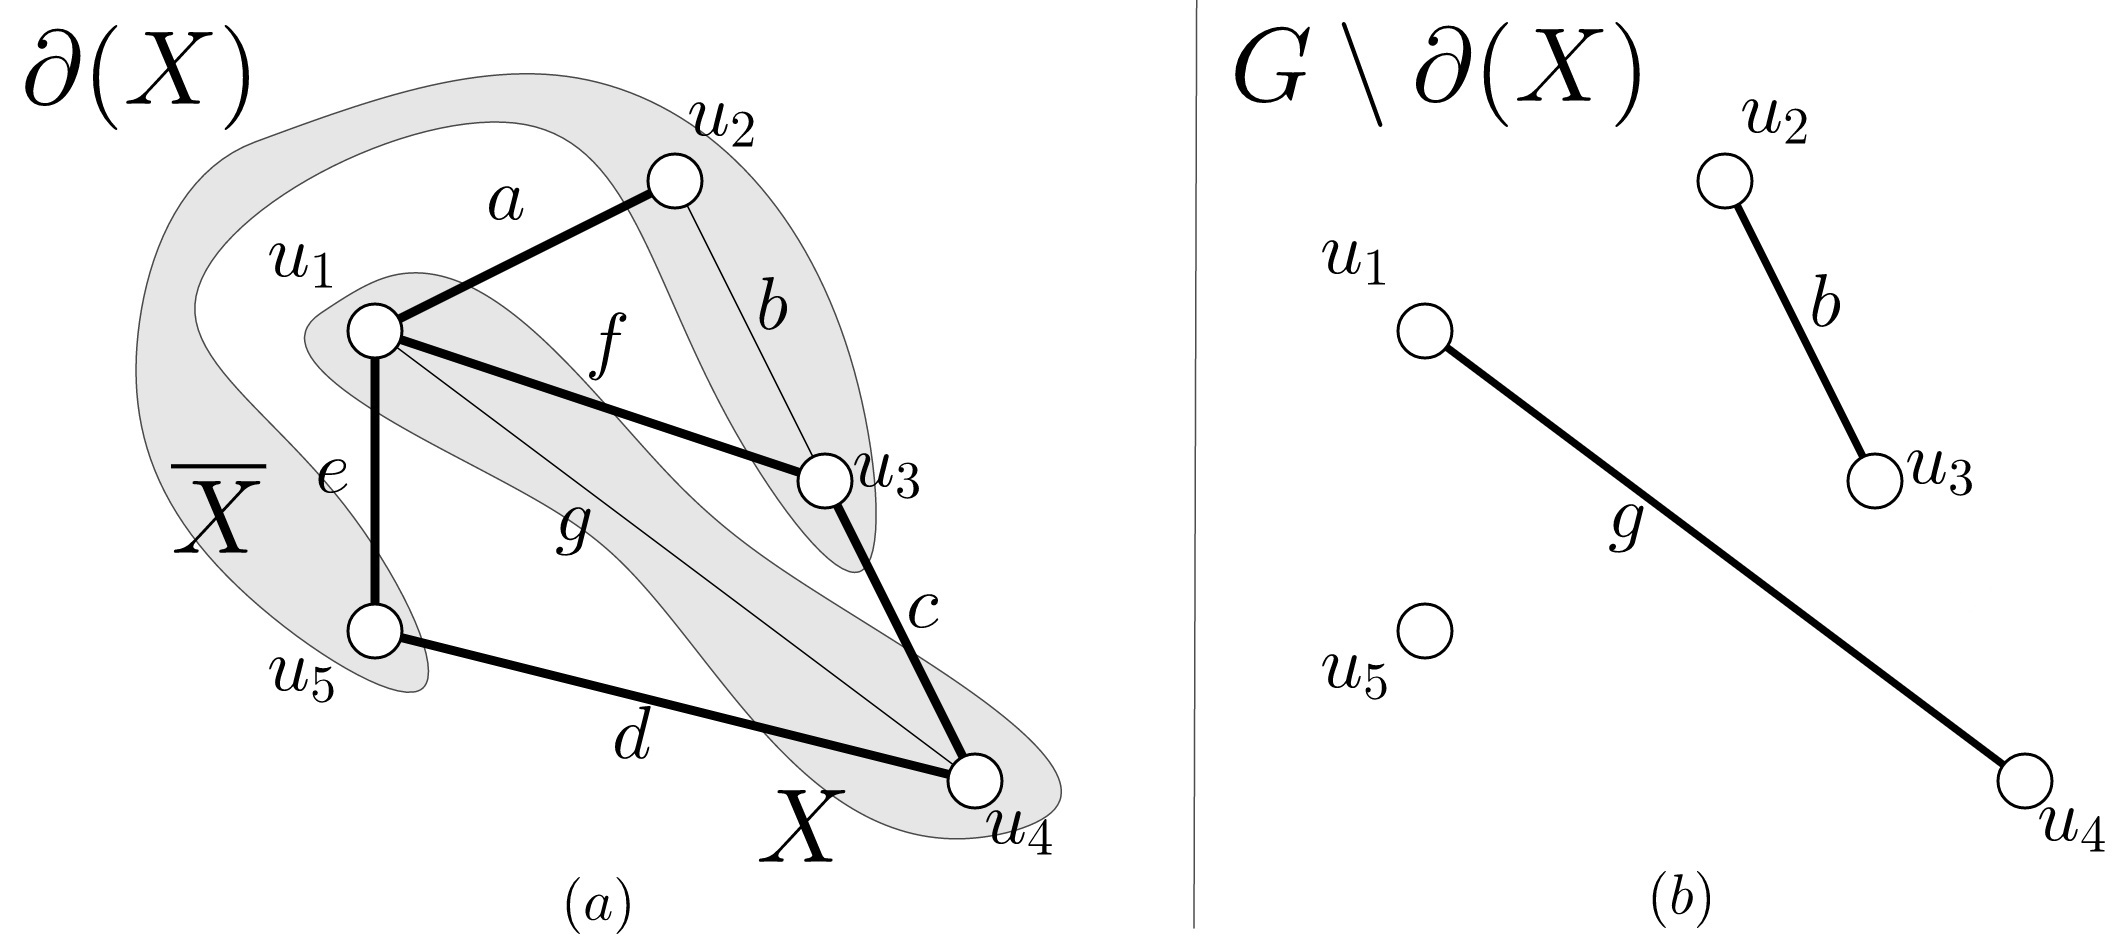
\includegraphics[scale=0.2]{img/imgchapter2/cortescompconexas.jpg}
     \caption{}
     \label{fig:cortescompconexas}
\end{figure}
\hfill $\blacklozenge$
\end{ejem}
\vspace{1cm}
\begin{ejem}
\begin{figure}[H]
    \centering
    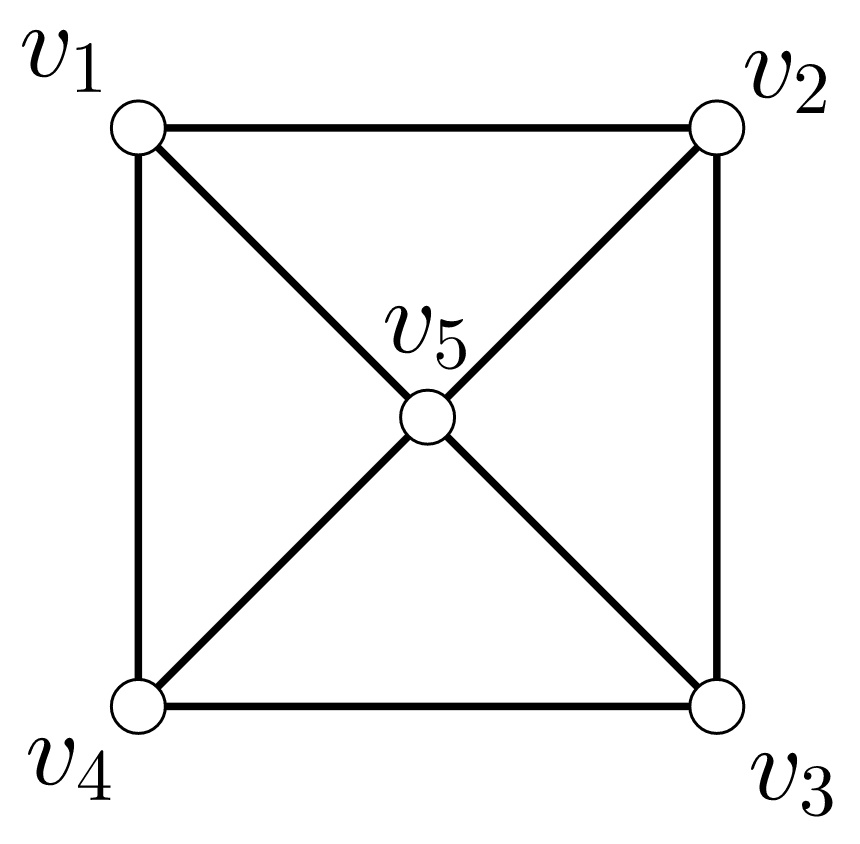
\includegraphics[scale=0.2]{img/imgchapter2/wheel.jpg}
    \caption{}
    \label{fig:wheel}
\end{figure}

Consideremos la gráfica \textit{rueda} $W_{4}$ de la figura \ref{fig:wheel}.
A continuación se muestra sus conjuntos de corte. Hemos resaltado los vértices respecto a los cuales se construye el corte en cuestión y las aristas de éste también se han remarcado. 

\begin{figure}[H]
    \centering
    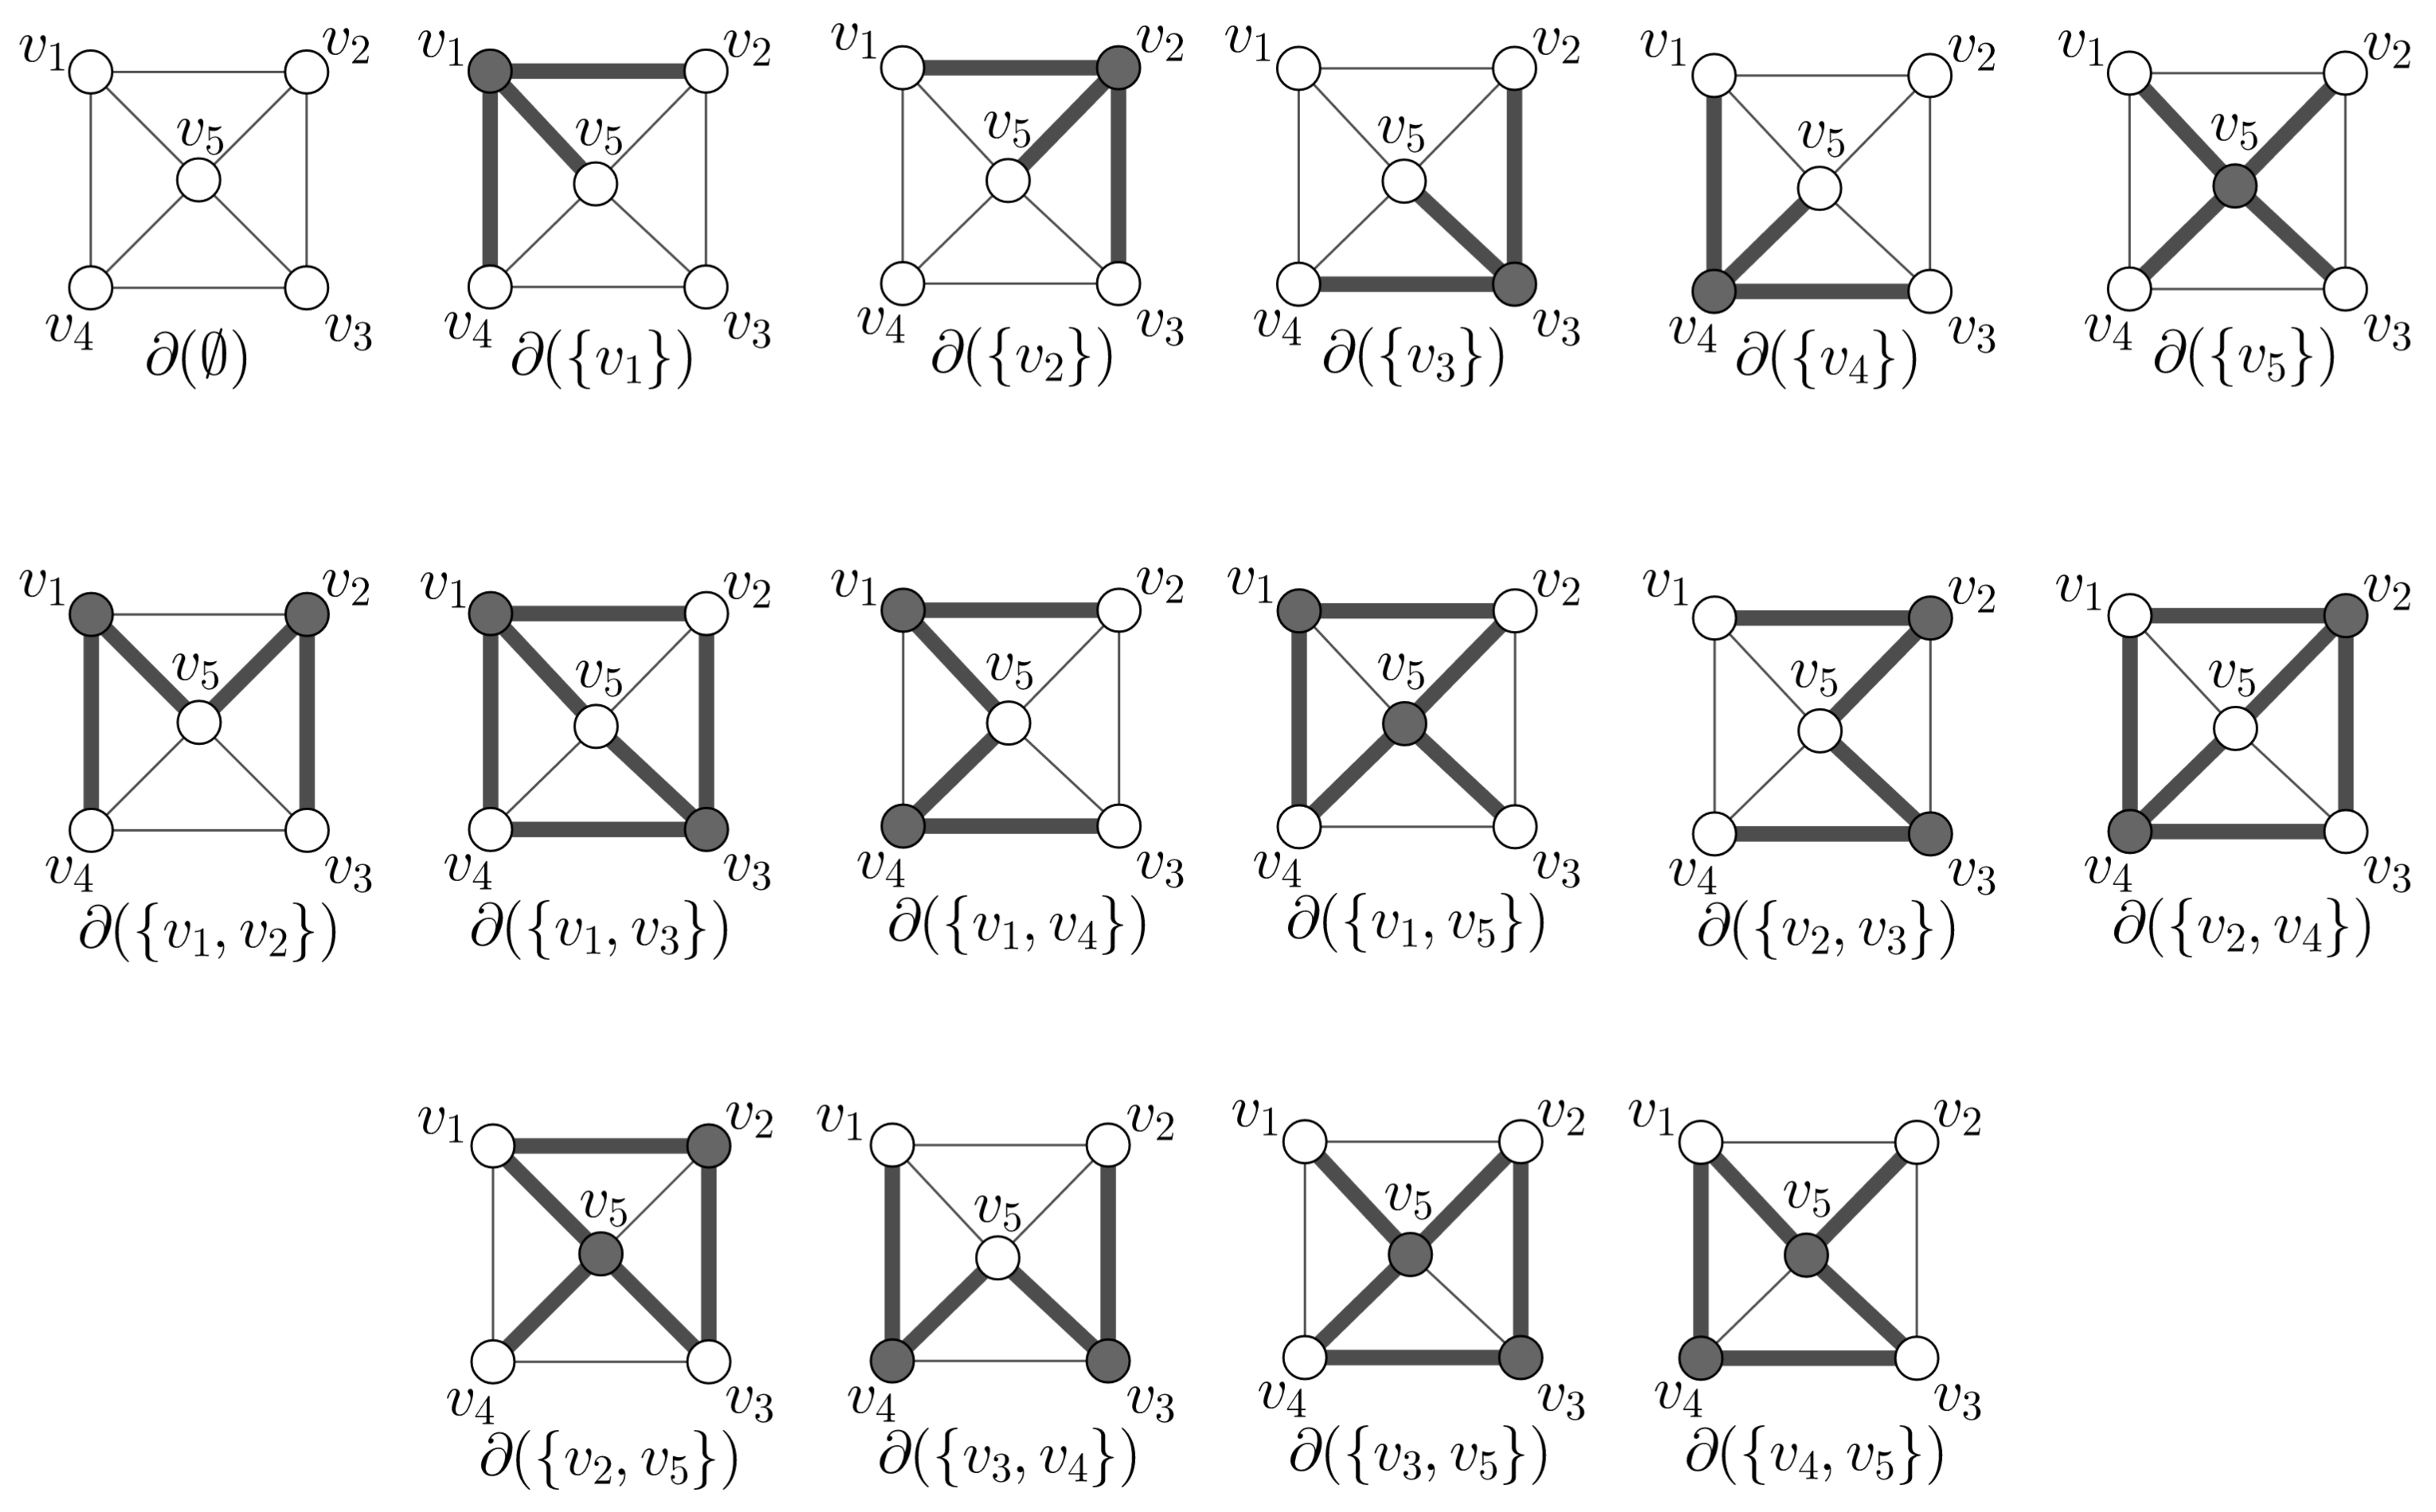
\includegraphics[scale=0.6]{img/imgchapter2/espaciocortes.jpg}
    \caption{Cortes de $W_{4}$}
    \label{fig:cortesw4}
\end{figure}

\hfill $\blacklozenge$
\end{ejem}

Analizaremos ahora las propiedades que tienen los conjuntos de corte:
%\vspace{1.5cm}
\begin{teo}\label{teo:diferenciasimetricacortes}
Sean $G$ una gráfica y  $X$ y $Y$ subconjuntos de $V(G)$. Entonces $$\partial(X) \triangle \partial(Y) = \partial(X \triangle Y).$$
\end{teo}

\begin{proof}
Recordemos que  
\begin{align*}
    X \triangle Y &= (X \cup Y)\setminus(X \cap Y) \\
                  &= (X \cup Y) \cap (\overline{X \cap Y})\\ 
                  &= (X \cup Y) \cap (\overline{X} \cup \overline{Y}).
\end{align*}

De esta última igualdad, tenemos que 
\begin{equation} \label{eq1}
    X \triangle Y = (\overline{X}\cap Y) \cup (X \cap \overline{Y}).
\end{equation}

Por otro lado,
\begin{align*}
    \overline{X \triangle Y} &= \overline{(X \cup Y) \cap (\overline{X \cap Y})} \\
                  &= \overline{X \cup Y} \cup (X \cap Y).
\end{align*}

 Así, llegamos a que
\begin{equation} \label{eq2}
   \overline{X \triangle Y} = (X \cap Y) \cup (\overline{X} \cap \overline{Y}).
\end{equation}
Como $V(G)=(X \triangle Y) \cup (\overline{X \triangle Y})$, de las igualdades \ref{eq1} y \ref{eq2} se sigue que 
\begin{equation} \label{eq3}
    V(G) = (X \cap Y) \cup (\overline{X} \cap \overline{Y}) \cup (\overline{X} \cap Y) \cup (X \cap \overline{Y}).
\end{equation}

El lado derecho de la igualdad \ref{eq3} sugiere que los cuatro conjuntos involucrados forman una partición de $V(G)$ (pues son ajenos dos a dos). Tomando en cuenta las definiciones de $\partial(X), \partial(Y)$ y  $\partial(X \triangle Y)$, en la figura \ref{fig:cortessim} se representa el comportamiento de estos conjuntos de corte con respecto a la partición del conjunto de vértices de $G$. En esta imagen, una línea remarcada simboliza un conjunto de aristas cuyos extremos están en algún subconjunto de vértices de la partición anterior.

\begin{figure}[H]
    \centering
    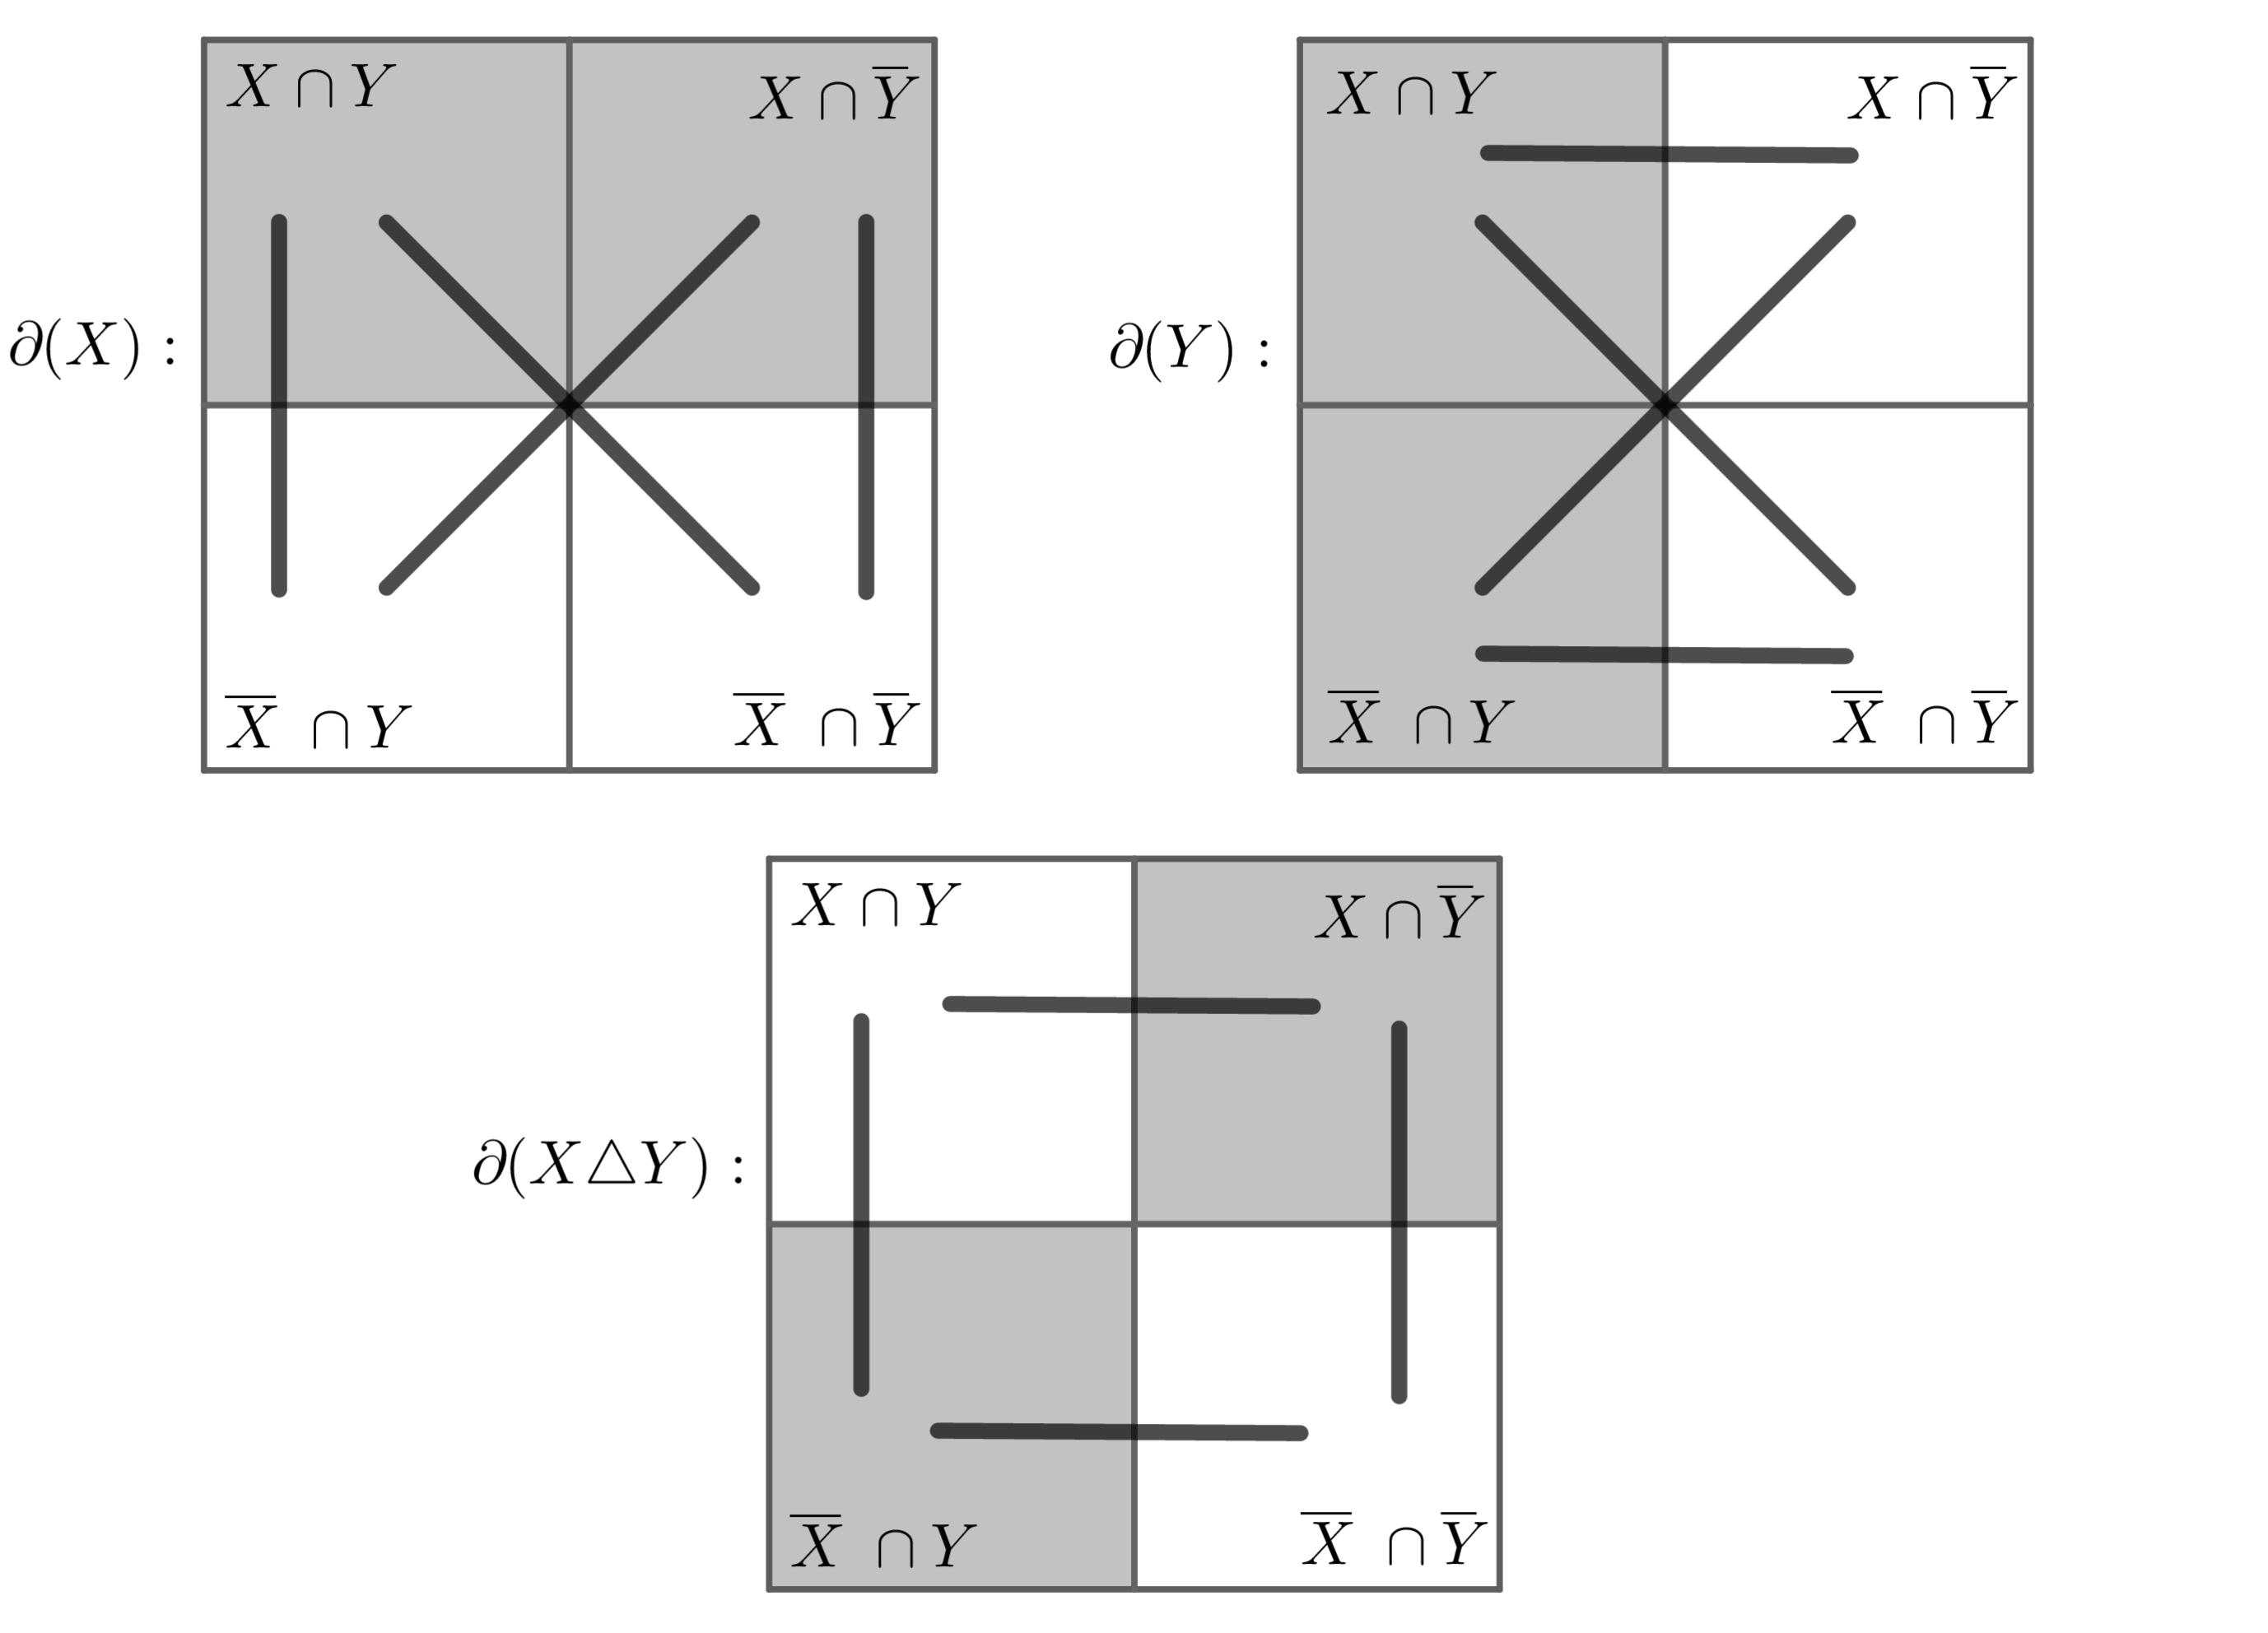
\includegraphics[width=0.75\textwidth]{img/imgchapter2/cortessim.jpg}
    \caption{Diferencia simétrica de dos conjuntos de corte}
    \label{fig:cortessim}
\end{figure}

Si, por simplicidad, hacemos 
\begin{align*}
    J &= \big ( E[X \cap Y, \overline{X} \cap Y] \big ) \bigcup \big(E[X \cap \overline{Y}, \overline{X} \cap \overline{Y}]\big), \\
    K &= \big(E[X \cap Y, X \cap \overline{Y}]\big) \bigcup \big(E[\overline{X} \cap Y, \overline{X} \cap \overline{Y}]\big), \\
    D &= \big(E[X \cap Y, \overline{X} \cap \overline{Y}]) \bigcup (E[X \cap \overline{Y}, \overline{X} \cap Y]\big),
\end{align*}
entonces es fácil darse cuenta (gracias a la figura \ref{fig:cortessim}) que $\partial(X)= J \cup D$, $ \partial(Y)= K \cup D$ y \\ $\partial(X \triangle Y)= J \cup K.$



Luego, observemos que 
\begin{align*}
    \partial(X) \triangle \partial(Y) &= (J \cup D) \triangle (K \cup D)\\ 
    &= (J \cup D) \triangle (K \cup D)\\ 
    &=  \big((J \cup D) \setminus (K \cup D)\big) \cup  \big((K \cup D) \setminus (J \cup D)\big)\\ 
    &= (J \setminus K) \cup (K \setminus J)\\
    & = J \cup K\\ 
    &= \partial(X \triangle Y).
\end{align*}

Las dos últimas igualdades sean porque los conjuntos de aristas que tomamos son ajenos mutuamente. En consecuencia, $\partial(X) \triangle \partial(Y) = \partial(X \triangle Y).$

\end{proof}

Por el Principio de Inducción, podemos generalizar el teorema anterior:
\begin{cor}\label{cor:cortessimInd}
Sean $G$ una gráfica y $X_{1},\ldots, X_{k}$ subconjuntos de $V(G)$. Entonces $$\difsym_{j=1}^{k} \partial(X_{j}) = \partial(\difsym_{j=1}^{k} X_{j}).$$
\end{cor}

Los resultados previos pueden expresarse en términos de subgráficas generadoras inducidas por los conjuntos de corte. En efecto, en el capítulo 1 vimos que la \textit{diferencia simétrica} de dos gráficas $G$ y $H$ es la gráfica $G \triangle H$, en la cual $V(G \triangle H) = V(G) \cup V(H)$ y $E(G \triangle H) = E(G)\triangle E(H)$. 

En particular, si $S_{1}$ y $S_{2}$ son subconjuntos de $E(G)$, tomemos las subgráficas generadoras inducidas $G[S_{1}]$ y $G[S_{2}]$. Entonces, por definición, el conjunto de aristas de la subgráfica generadora  $G[S_{1}] \triangle G[S_{2}]$ es $S_{1} \triangle S_{2}$. Al mismo tiempo, éste es también el conjunto de aristas de la subgráfica generadora inducida $G[S_{1} \triangle S_{2}]$. Como ambas subgráficas tienen el mismo conjunto de vértices (pues son generadoras), obtenemos que 
$$G[S_{1}] \triangle G[S_{2}] = G[S_{1} \triangle S_{2}].$$ 
Claramente, la igualdad anterior puede extenderse a una cantidad finita arbitraria de subconjuntos de aristas de $G$. Luego, gracias al corolario \ref{cor:cortessimInd} podemos afirmar que
$$
G\Big[\difsym_{j=1}^{k} \partial(X_{j})\Big] = G\Big[\partial(\difsym_{j=1}^{k} X_{j})\Big].
$$

Por lo que argumentamos líneas arriba, sabemos que $G\Big[\difsym_{j=1}^{k} \partial(X_{j})\Big] = \difsym_{j=1}^{k}G\Big[ \partial(X_{j})\Big]$. Obtenemos de esta forma el siguiente corolario:

\begin{cor}\label{cor:difsimGeneradora}
Sean $G$ una gráfica y $X_{1},\ldots, X_{k}$ subconjuntos de $V(G)$. Entonces $$\difsym_{j=1}^{k}G\Big[ \partial(X_{j})\Big] = G\Big[\partial(\difsym_{j=1}^{k} X_{j})\Big].$$
\end{cor}

Veamos ahora otro resultado y su generalización, similares al teorema \ref{teo:diferenciasimetricacortes} y al corolario \ref{cor:cortessimInd}.

\begin{prop} \label{prop2}
Sean $H_{1}$ y $H_{2}$ subgráficas de $G$. Si $X \subseteq V(G)$, entonces 
$$
\partial_{H_{1} \triangle H_{2}}(X) = \partial_{H_{1}}(X) \triangle \partial_{H_{2}}(X).
$$
\end{prop}

\begin{proof} Lo haremos por \textit{doble contención}. Para la primer contención, tomamos $a$ en $\partial_{H_{1} \triangle H_{2}}(X)$. Entonces la arista $a$ es adyacente a dos vértices: $u$ y $v$; asumiremos (sin pérdida de generalidad) que el primero está en $X$ y el otro en $\overline{X}$. Entonces $a \in E(H_{1} \triangle H_{2})=E(H_{1}) \triangle E(H_{2})$. Si $a$ está en $E(H_{1})$ (y no a $E(H_{2})$), necesariamente $a$ pertenece a $\partial_{H_{1}}(X)$ por cómo son los vértices de $a$. No sucede que $a \in \partial_{H_{2}}(X)$ porque $a \notin E(H_{2})$. 

Análogamente, si $a$ es elemento de $E(H_{2})$ (y no de $E(H_{1})$), entonces $a \in \partial_{H_{2}}(X)$ y no pertenece a $\partial_{H_{1}}(X)$. Por tanto, $a \in \partial_{H_{1}}(X) \triangle \partial_{H_{2}}(X)$. De esta manera, hallamos que $$\partial_{H_{1} \triangle H_{2}}(X) \subseteq \partial_{H_{1}}(X) \triangle \partial_{H_{2}}(X).$$

Ahora suponemos que la arista $a$ pertenece al conjunto $\partial_{H_{1}}(X) \triangle \partial_{H_{2}}(X)$. Por la definición de la \textit{diferencia simétrica} existen dos casos.
\begin{itemize}
    \item \underline{Caso 1}: Supongamos que $a$ pertenece a $\partial_{H_{1}}(X)$ (y, por tanto, no es elemento de $\partial_{H_{2}}(X)$). Entonces $a \in E(H_{1})$. No es posible que $a \in E(H_{2})$, pues, inmediatamente, $a$ estaría en $\partial_{H_{2}}(X)$ (ya que $u \in X$ y $v \in \overline{X}$), y, por lo tanto, es una contradicción. Por consiguiente, $$a \in E(H_{1}) \triangle E(H_{2}) = E(H_{1} \triangle H_{2}).$$ Dado que un extremo de la arista está en $X$ y el otro en el complemento de $X$, deducimos que $a \in \partial_{H_{1} \triangle H_{2}}(X)$.
    
    \item \underline{Caso 2}: Supongamos que $a$ pertenece a $\partial_{H_{2}}(X)$ (y, por tanto, no es elemento de $\partial_{H_{1}}(X)$). Procediendo de forma análoga al caso anterior obtenemos, también, que $a \in \partial_{H_{1} \triangle H_{2}}(X)$.
\end{itemize}
De ambos casos, afirmamos que $\partial_{H_{1}}(X) \triangle \partial_{H_{2}}(X) \subseteq \partial_{H_{1} \triangle H_{2}}(X)$ y concluimos, pues, que $$\partial_{H_{1} \triangle H_{2}}(X) = \partial_{H_{1}}(X) \triangle \partial_{H_{2}}(X).$$

\end{proof}

\begin{cor}\label{cor:cortessimIndSubgrafica}
Sean $H_{1},\ldots, H_{k}$ subgráficas de $G$. Entonces $$\partial_{H_{1} \triangle \cdots \triangle H_{k}}(X) =\partial_{H_{1}}(X) \triangle \cdots \triangle H_{k}(X) .$$ 
\end{cor}


Por último, antes de continuar a la siguiente subsección, comentaremos un poco sobre los conjuntos de corte en una gráfica $G$ inconexa. Supongamos que $F_{1}, \ldots, F_{c}$ son sus componentes conexas y que $c:=c(G)$. Entonces $G = \bigcup_{i=1}^{c}F_{i}$. Nótese que esta es una unión ajena de gráficas, por lo que también podemos expresarla así:
$$G=\difsym_{j=1}^{c} F_{j}.$$

 Tomemos $X \subseteq V(G)$. Luego,
 \begin{align*}
   \partial_{G}(X) &= \partial_{F_{1} \triangle \cdots \triangle F_{c}}(X) \\
   &= \partial_{F_{1}}(X) \triangle \ldots \triangle \partial_{F_{1}}(X) \textnormal{ (por el corolario \ref{cor:cortessimIndSubgrafica})}\\
   &= \bigcup_{j=1}^{c}\partial_{F_{j}}(X) \textnormal{ (por que la unión es ajena).}
 \end{align*}
 
    Por otro lado, haciendo $X_{i}:=X \cap V(F_{i})$, con $i \in \{1, \ldots, c\}$, es claro que $\bigcup_{j=1}^{c}X_{j} = X$ y  deducimos que
    \begin{align*}
        \partial_{F_{i}}(X) &= \partial_{F_{i}}(\bigcup_{j=1}^{c}X_{j})\\
        &=\partial_{F_{i}}(\difsym_{j=1}^{c}X_{j}) \textnormal{ (la unión es ajena)}\\
        &= \difsym_{j=1}^{c} \partial_{F_{i}}(X_{j}) \textnormal{ (por el corolario \ref{cor:cortessimInd})}.
    \end{align*}
     Si $i \neq j$, $\partial_{F_{i}}(X_{j}) = \emptyset$ porque $\partial_{F_{i}}(X_{j}) \subseteq E(F_{i})$ y $X_{j} \subseteq V(F_{j})$, pero no hay aristas que conecten vértices de diferentes componente conexas. Por lo tanto, $\partial_{F_{i}}(X) = \partial_{F_{i}}(X_{i})$ y $\partial_{G}(X) = \bigcup_{j=1}^{c}\partial_{F_{j}}(X_{j})$.
    
    
    La figura siguiente representa la situación anterior:
 \begin{figure}[H]
    \centering
    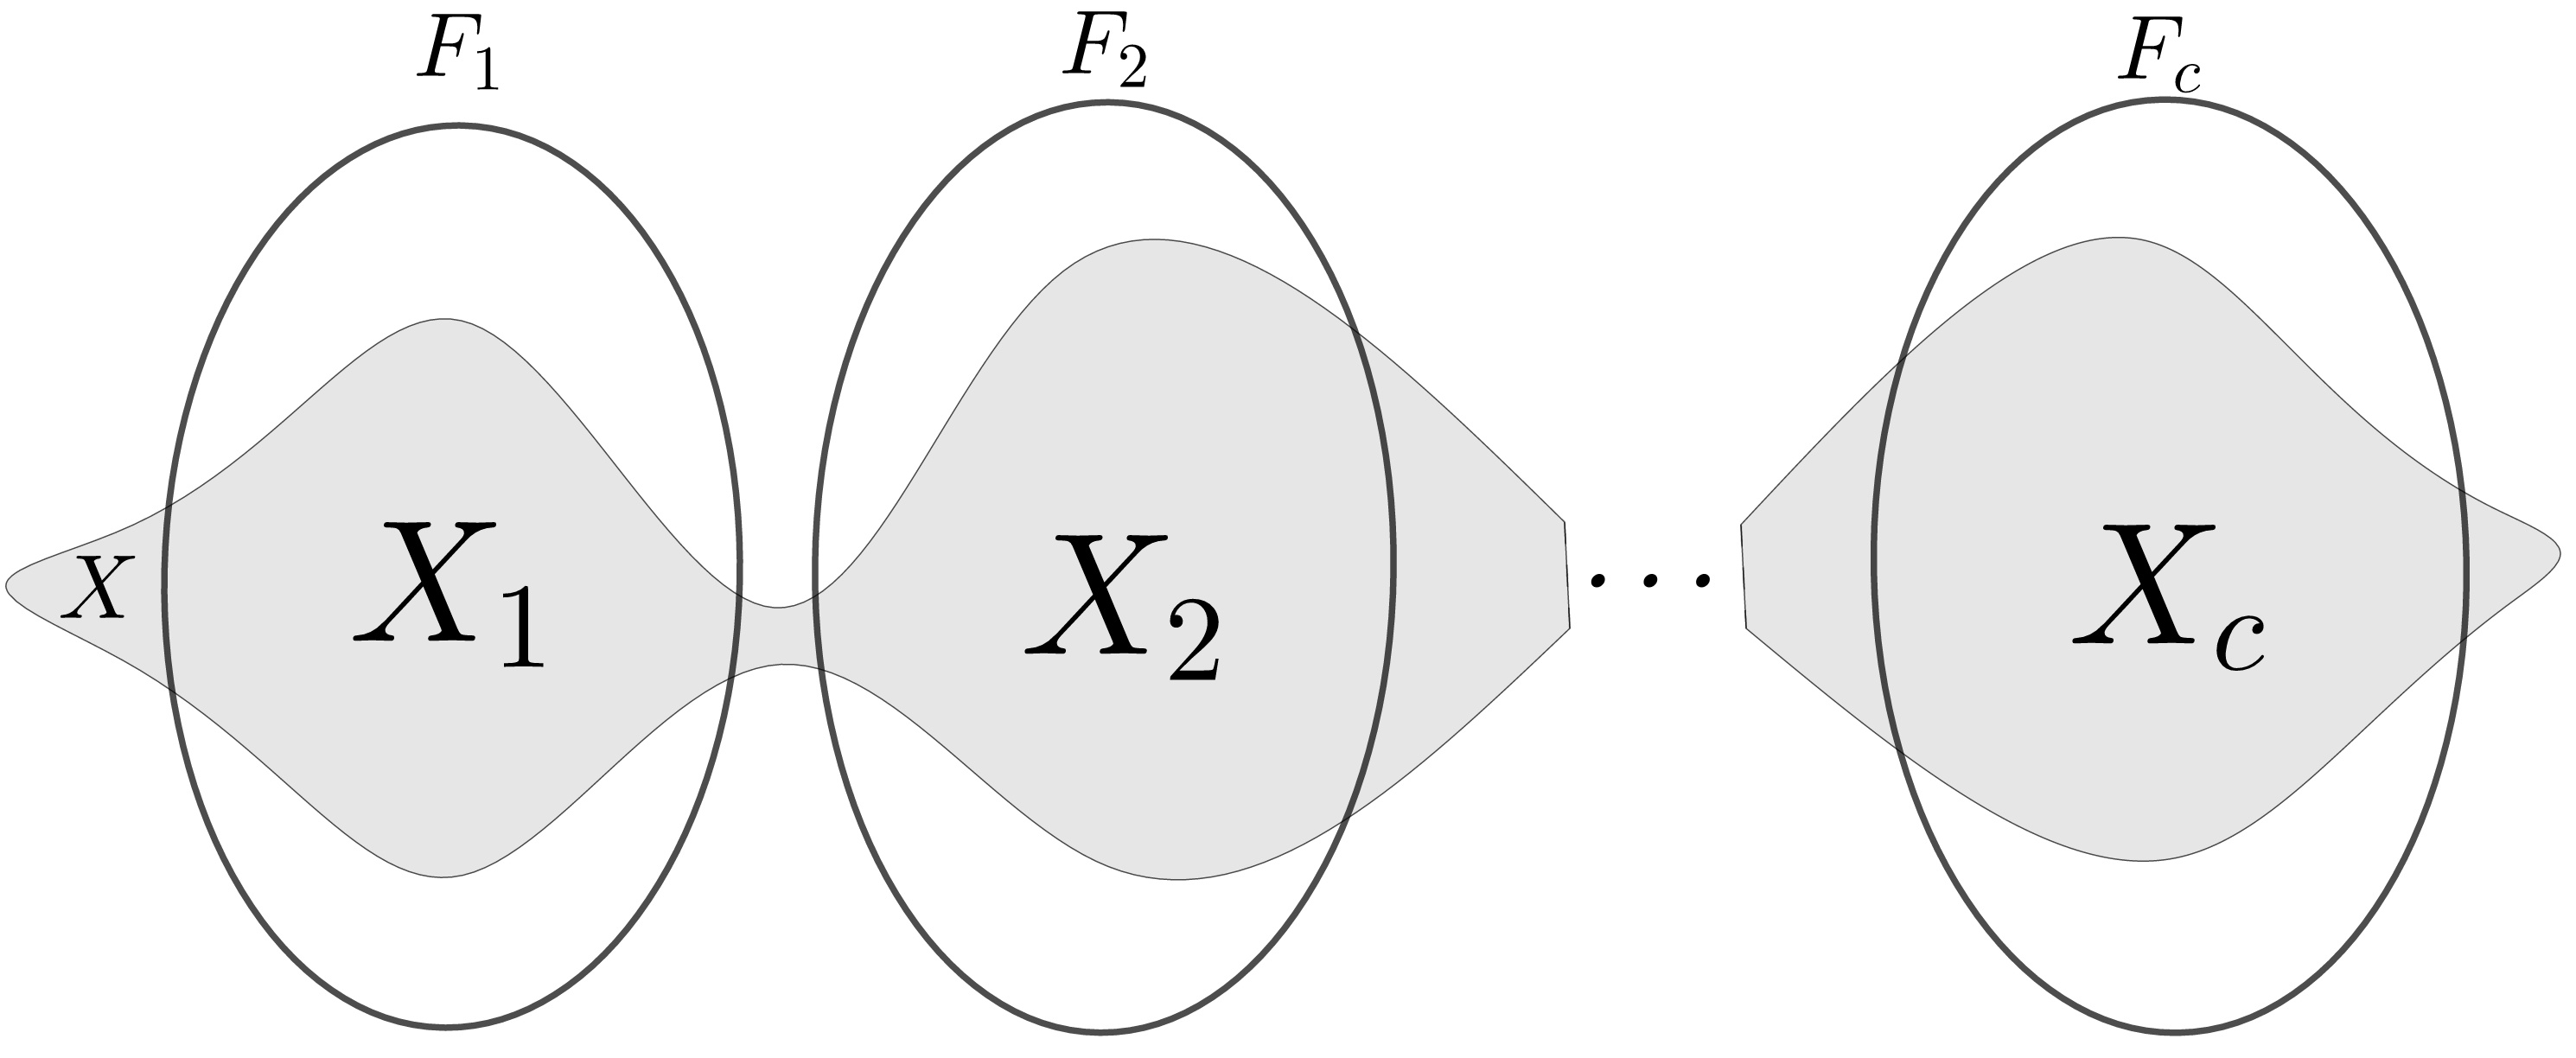
\includegraphics[scale=0.15]{img/imgchapter2/componentes.jpg}
    \caption{}
    \label{fig:componentes}
\end{figure}

\subsection{Conjuntos de corte minimales}

Llamamos \textit{conjunto de corte minimal de} \index{Conjunto de corte! minimal} $G$ (en \cite{Bondy}, los autores le llaman \textit{bond}) a un conjunto de corte no vacío con la propiedad de que ninguno de sus subconjuntos propios, no vacíos, es otro conjunto de corte. Esto implica que, $B$ es un corte minimal de $G$ y $S$ es un conjunto de corte tal que $S\subseteq B$, necesariamente $B=S$.

 En general, un conjunto de corte \textit{divide} a $G$ en, al menos, dos componentes conexas. No obstante, el teorema siguiente nos asegura que los cortes minimales son aquellos que dividen a una gráfica conexa en, \textit{exactamente}, dos componentes. Recuérdese que $G[X]$ es la gráfica inducida por el conjunto de vértices $X$.

\begin{teo} \label{teo:caracterizacionbond}
Sean $G$ una gráfica conexa y $X$ un subconjunto de vértices de $G$, de tal manera que $\partial(X) \neq \emptyset$. Entonces $\partial(X)$ es un conjunto de corte minimal si y sólo si $G[X]$ y $G[\bar{X}]$ son conexas. 
\end{teo}

\begin{proof} Asumimos que $G$ es conexa y que $X \subseteq V(G)$. Probaremos la necesidad por contrapositiva. Supóngase primero que $G[X]$ no es conexa. Entonces existe una partición de $X$ en dos conjuntos, no vacíos, entre los cuales no hay aristas; en otros términos, existe $Y \neq \emptyset$ tal que $Y \subsetneqq X$ y $X \setminus Y \subsetneqq X$, cumpliendo $E\big[Y, X \setminus Y \big] = E\big[X \cap Y, X \cap \overline{Y} \big] = \emptyset$. Además, dado que $Y \subsetneqq X$, se cumple también que $\overline{X} \cap Y = \emptyset$.

Retomando las ideas de la prueba del teorema \ref{teo:diferenciasimetricacortes} (compárense las figuras \ref{fig:cortessim} y \ref{fig:bond2}) y dada la información del párrafo anterior, deducimos que $$\partial(Y) = E[X \cap Y, \overline{X} \cap \overline{Y}] \text{ y } \partial(X) = \big(E[X \cap \overline{Y}, \overline{X} \cap \overline{Y}]\big) \bigcup \big(E[X \cap Y, \overline{X} \cap \overline{Y}]\big).$$ Así, es claro que $\partial (Y) \subseteq \partial(X)$. Se mencionó previamente que en una gráfica conexa ningún conjunto de corte puede ser vacío. Luego, la conexidad de $G$ garantiza que $\partial(Y) \neq \emptyset$.

\begin{figure}[H]
    \centering
    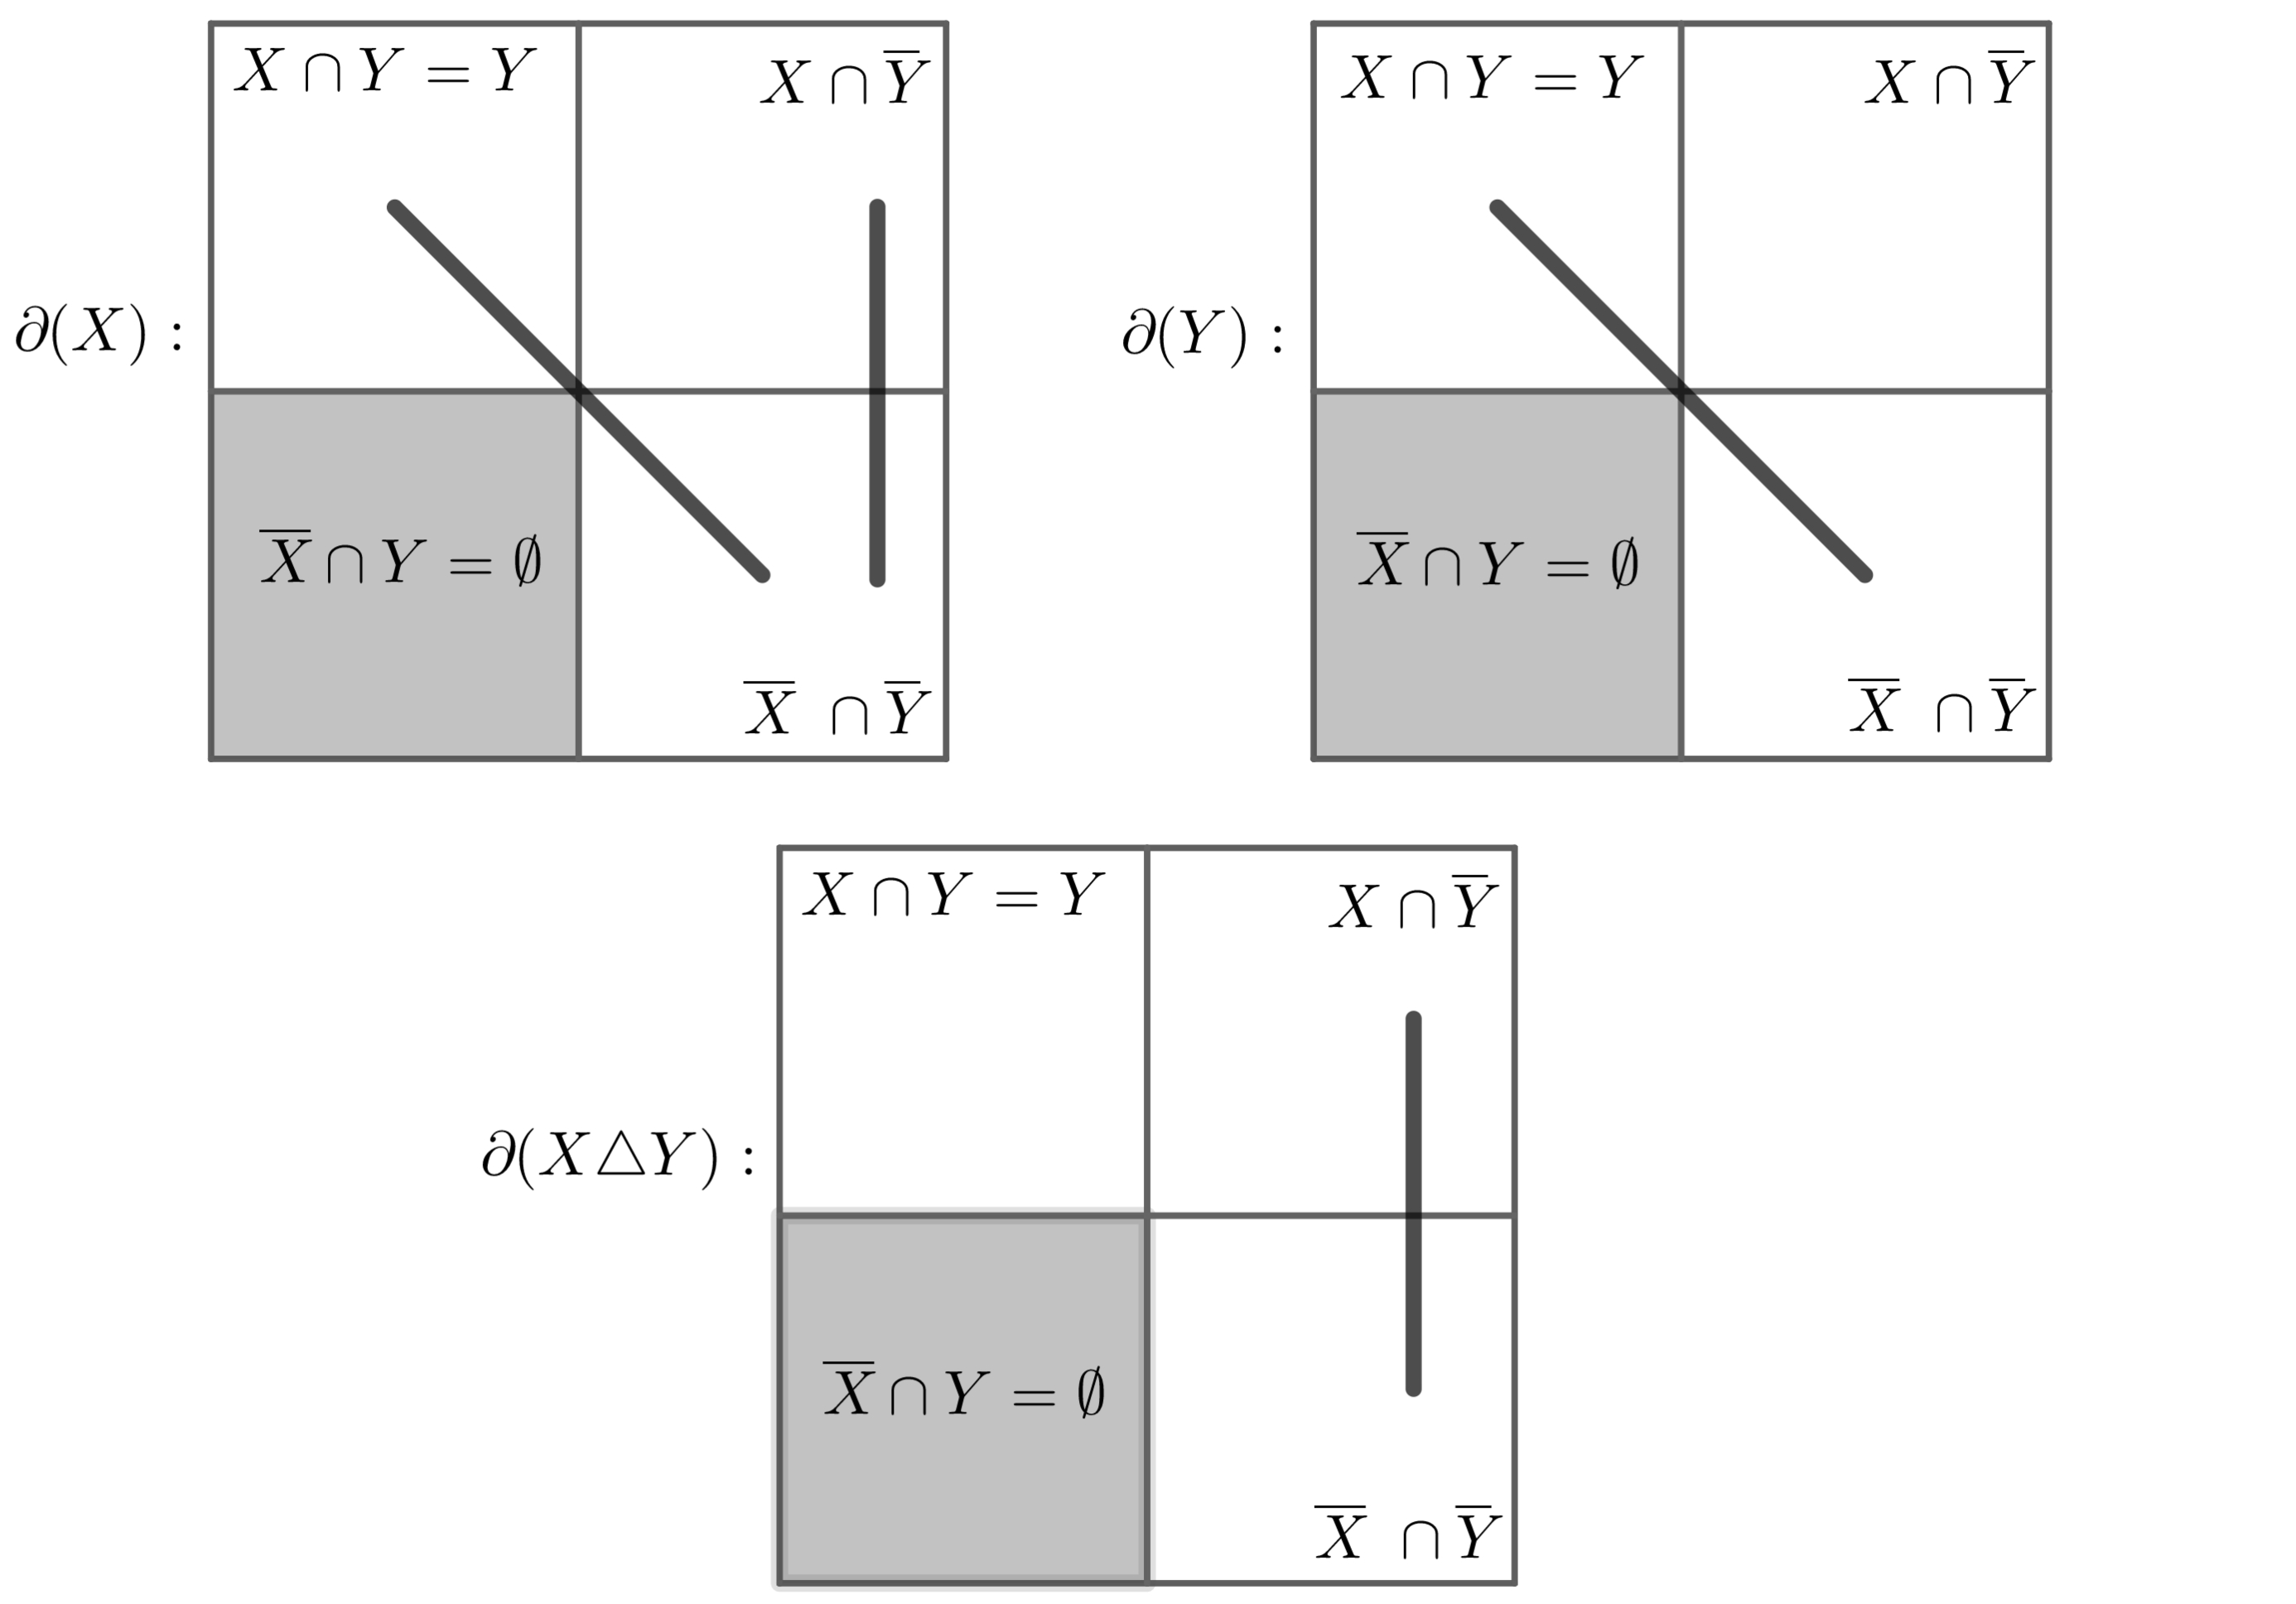
\includegraphics[scale=0.6]{img/imgchapter2/bond2.jpg}
    \caption{}
    \label{fig:bond2}
\end{figure}
Además, por el teorema \ref{teo:diferenciasimetricacortes}, $\partial(X \triangle Y)= \partial(X) \triangle \partial(Y)$. Entonces, como se muestra en la figura \ref{fig:bond2}, $\partial(X \triangle Y) = E[X \cap \overline{Y}, \overline{X} \cap \overline{Y}]$. Una vez más, la conexidad de $G$ asegura que $\partial(X \triangle Y) \neq \emptyset$. Así, en efecto, $E[X \cap \overline{Y}, \overline{X} \cap \overline{Y}] \neq \emptyset$. Esta última afirmación implica que $\partial(Y) \subsetneqq \partial(X)$. Por consiguiente, $\partial(X)$ no es un conjunto de corte minimal pues contiene propiamente a otro conjunto de corte no vacío. Si, en segundo lugar, suponemos que $G[\bar{X}]$ no es conexa, mediante razonamientos similares podremos concluir también que $\partial(X)$ no es un conjunto de corte minimal.


La suficiencia se prueba por contradicción. Supóngase, pues, que $G[X]$ y $G[\bar{X}]$ son conexas y que $\partial(X)$ no es un conjunto de corte minimal. Entonces existe $Y \subseteq V(G)$ tal que $\partial(Y) \subsetneqq \partial(X)$ y $\partial(Y) \neq \emptyset$. Nótese que este último hecho implica que (ver la figura \ref{fig:cortessim}) $$\partial(Y)= \big(E[X \cap Y, \overline{X} \cap \overline{Y}]) \bigcup (E[X \cap \overline{Y}, \overline{X} \cap Y]\big),$$ de donde $$E[X \cap Y, X \cap \overline{Y}] = \emptyset = E[\overline{X} \cap Y, \overline{X} \cap \overline{Y}].$$ 

Recordemos que, para llegar a una contradicción, necesitamos argumentar que $G[X]$ es inconexa ó $G[\bar{X}]$ es inconexa, encontrando alguna partición de sus conjuntos de vértices, de tal manera que no haya aristas entre los conjuntos de la partición. 

Lo haremos analizando las cuatro intersecciones que aparecen en la última igualdad. Éstos formarán las particiones que buscamos, pero debemos confirmar que los conjuntos son no vacíos. Hasta aquí nada nos garantiza que alguna de ellos sea distinto del conjunto vacío. Pero tenemos dos casos: que la intersección de $X$ con $Y$ sea vacía o que no lo sea.   


\begin{itemize}
    \item \underline{Caso 1}. Asumimos que $X \cap Y = \emptyset$. Veamos que $(\overline{X} \cap Y, \overline{X} \cap \overline{Y})$ es una partición del conjunto de vértices $\overline{X}$.
    
    Como $X \cap Y = \emptyset$, entonces $Y \subseteq \overline{X}$ y, en consecuencia, $\overline{X} \cap Y = Y$. Dado que $\partial(Y) \neq \emptyset$, entonces $Y$ es no vacío (porque al menos hay una arista con un extremo en $Y$). Como $\overline{X} \cap Y = Y$, deducimos que $\overline{X} \cap Y \neq \emptyset$.
    
    Por otra parte, no podría suceder que $\overline{X} \cap \overline{Y} = \emptyset$, pues tendríamos que $\overline{X} \subseteq Y$, es decir, $\overline{X} = Y$ y, por tanto, $\partial(Y) = \partial(\overline{X})=\partial(X)$, lo cual es una contradicción. Así, necesariamente, $\overline{X} \cap \overline{Y} \neq \emptyset$

    En resumen, sabemos que $\overline{X} \cap Y \neq \emptyset$, $\overline{X} \cap \overline{Y} \neq \emptyset$. Por lo tanto, $(\overline{X} \cap Y, \overline{X} \cap \overline{Y})$ es una partición de $\overline{X}$.
    
    No obstante, ya vimos que  $E[\overline{X} \cap Y, \overline{X} \cap \overline{Y}] = \emptyset$, es decir, no hay aristas entre los miembros de la partición de $\overline{X}$. Esto implicaría que $G[\bar{X}]$ no es conexa, y contradice nuestras hipótesis.
    
    \item \underline{Caso 2}. Suponemos que $X \cap Y \neq \emptyset$. 
    
    Si se cumpliera que $X \cap \overline{Y} \neq \emptyset$, $G[X]$ no sería conexa pues $(X \cap Y, X \cap \overline{Y})$ es una partición de $X$ y $E[X \cap Y, X \cap \overline{Y}] = \emptyset$, lo cual, de nuevo, es una contradicción. 
    
    Entonces debe cumplirse que $X \cap \overline{Y} = \emptyset$, o sea, que $\overline{Y} \subseteq \overline{X}$. La consecuencia de esta última afirmación es que tanto $\overline{X} \cap Y$ como $\overline{X} \cap \overline{Y}$ son conjuntos distintos del vacío. 

    En efecto, si $\overline{X} \cap Y = \emptyset$ sabemos que $\overline{X} \subseteq \overline{Y}$. Dado que $\overline{Y} \subseteq \overline{X}$, entonces $Y = X$ y $\partial(Y) = \partial(X)$, lo cual es imposible. Por otro lado, si se diera que $\overline{X} \cap \overline{Y} = \emptyset$, tendríamos que $\overline{Y} \subseteq X$. Como $\overline{Y} \subseteq \overline{X}$, también $X \subseteq Y$. Por consiguiente, $\overline{Y} \subseteq Y$. Esto último implica que $Y=V$, pero es falso debido a que $\partial(Y) = \partial(V) = \emptyset$, y se vio desde antes que $\partial(Y)\neq \emptyset$.

    En resumen, sabemos que $\overline{X} \cap Y \neq \emptyset$, $\overline{X} \cap \overline{Y} \neq \emptyset$. Por lo tanto, $(\overline{X} \cap Y, \overline{X} \cap \overline{Y})$ es una partición de $\overline{X}$. Ya sabemos que $E[\overline{X} \cap Y, \overline{X} \cap \overline{Y}] = \emptyset$, es decir, no hay aristas entre los miembros de la partición de $\overline{X}$. Esto implicaría que $G[\bar{X}]$ no es conexa, y contradice, de nuevo, nuestras hipótesis.
\end{itemize}


Podemos asegurar que los casos anteriores no son posibles. Las dificultades surgieron a partir de suponer que $\partial(X)$ no es un conjunto de corte minimal. Concluimos, entonces, que $\partial(X)$ es un conjunto de corte minimal si y sólo si $G[X]$ y $G[\bar{X}]$ son conexas. 

\end{proof}

Es sencillo darse cuenta que el teorema \ref{teo:caracterizacionbond} implica el siguiente corolario.

\begin{cor}\label{cor:corteminimalcomponentesconexas}
 Si $G$ es una gráfica conexa y $X\subseteq V(G)$, entonces $\partial(X)$ es un conjunto de corte minimal si y sólo si $G\setminus \partial(X)$ tiene exactamente dos componentes conexas. 
\end{cor}


\begin{ejem}
En la figura que se muestra a continuación están todos los conjuntos de corte minimales de la gráfica $W_{4}$. Observe que si retiráramos de $W_{4}$ las aristas de cualquiera de estos conjuntos de corte, nos quedarían dos componentes conexas, como lo asegura el teorema anterior.

\begin{figure}[H]
    \centering
    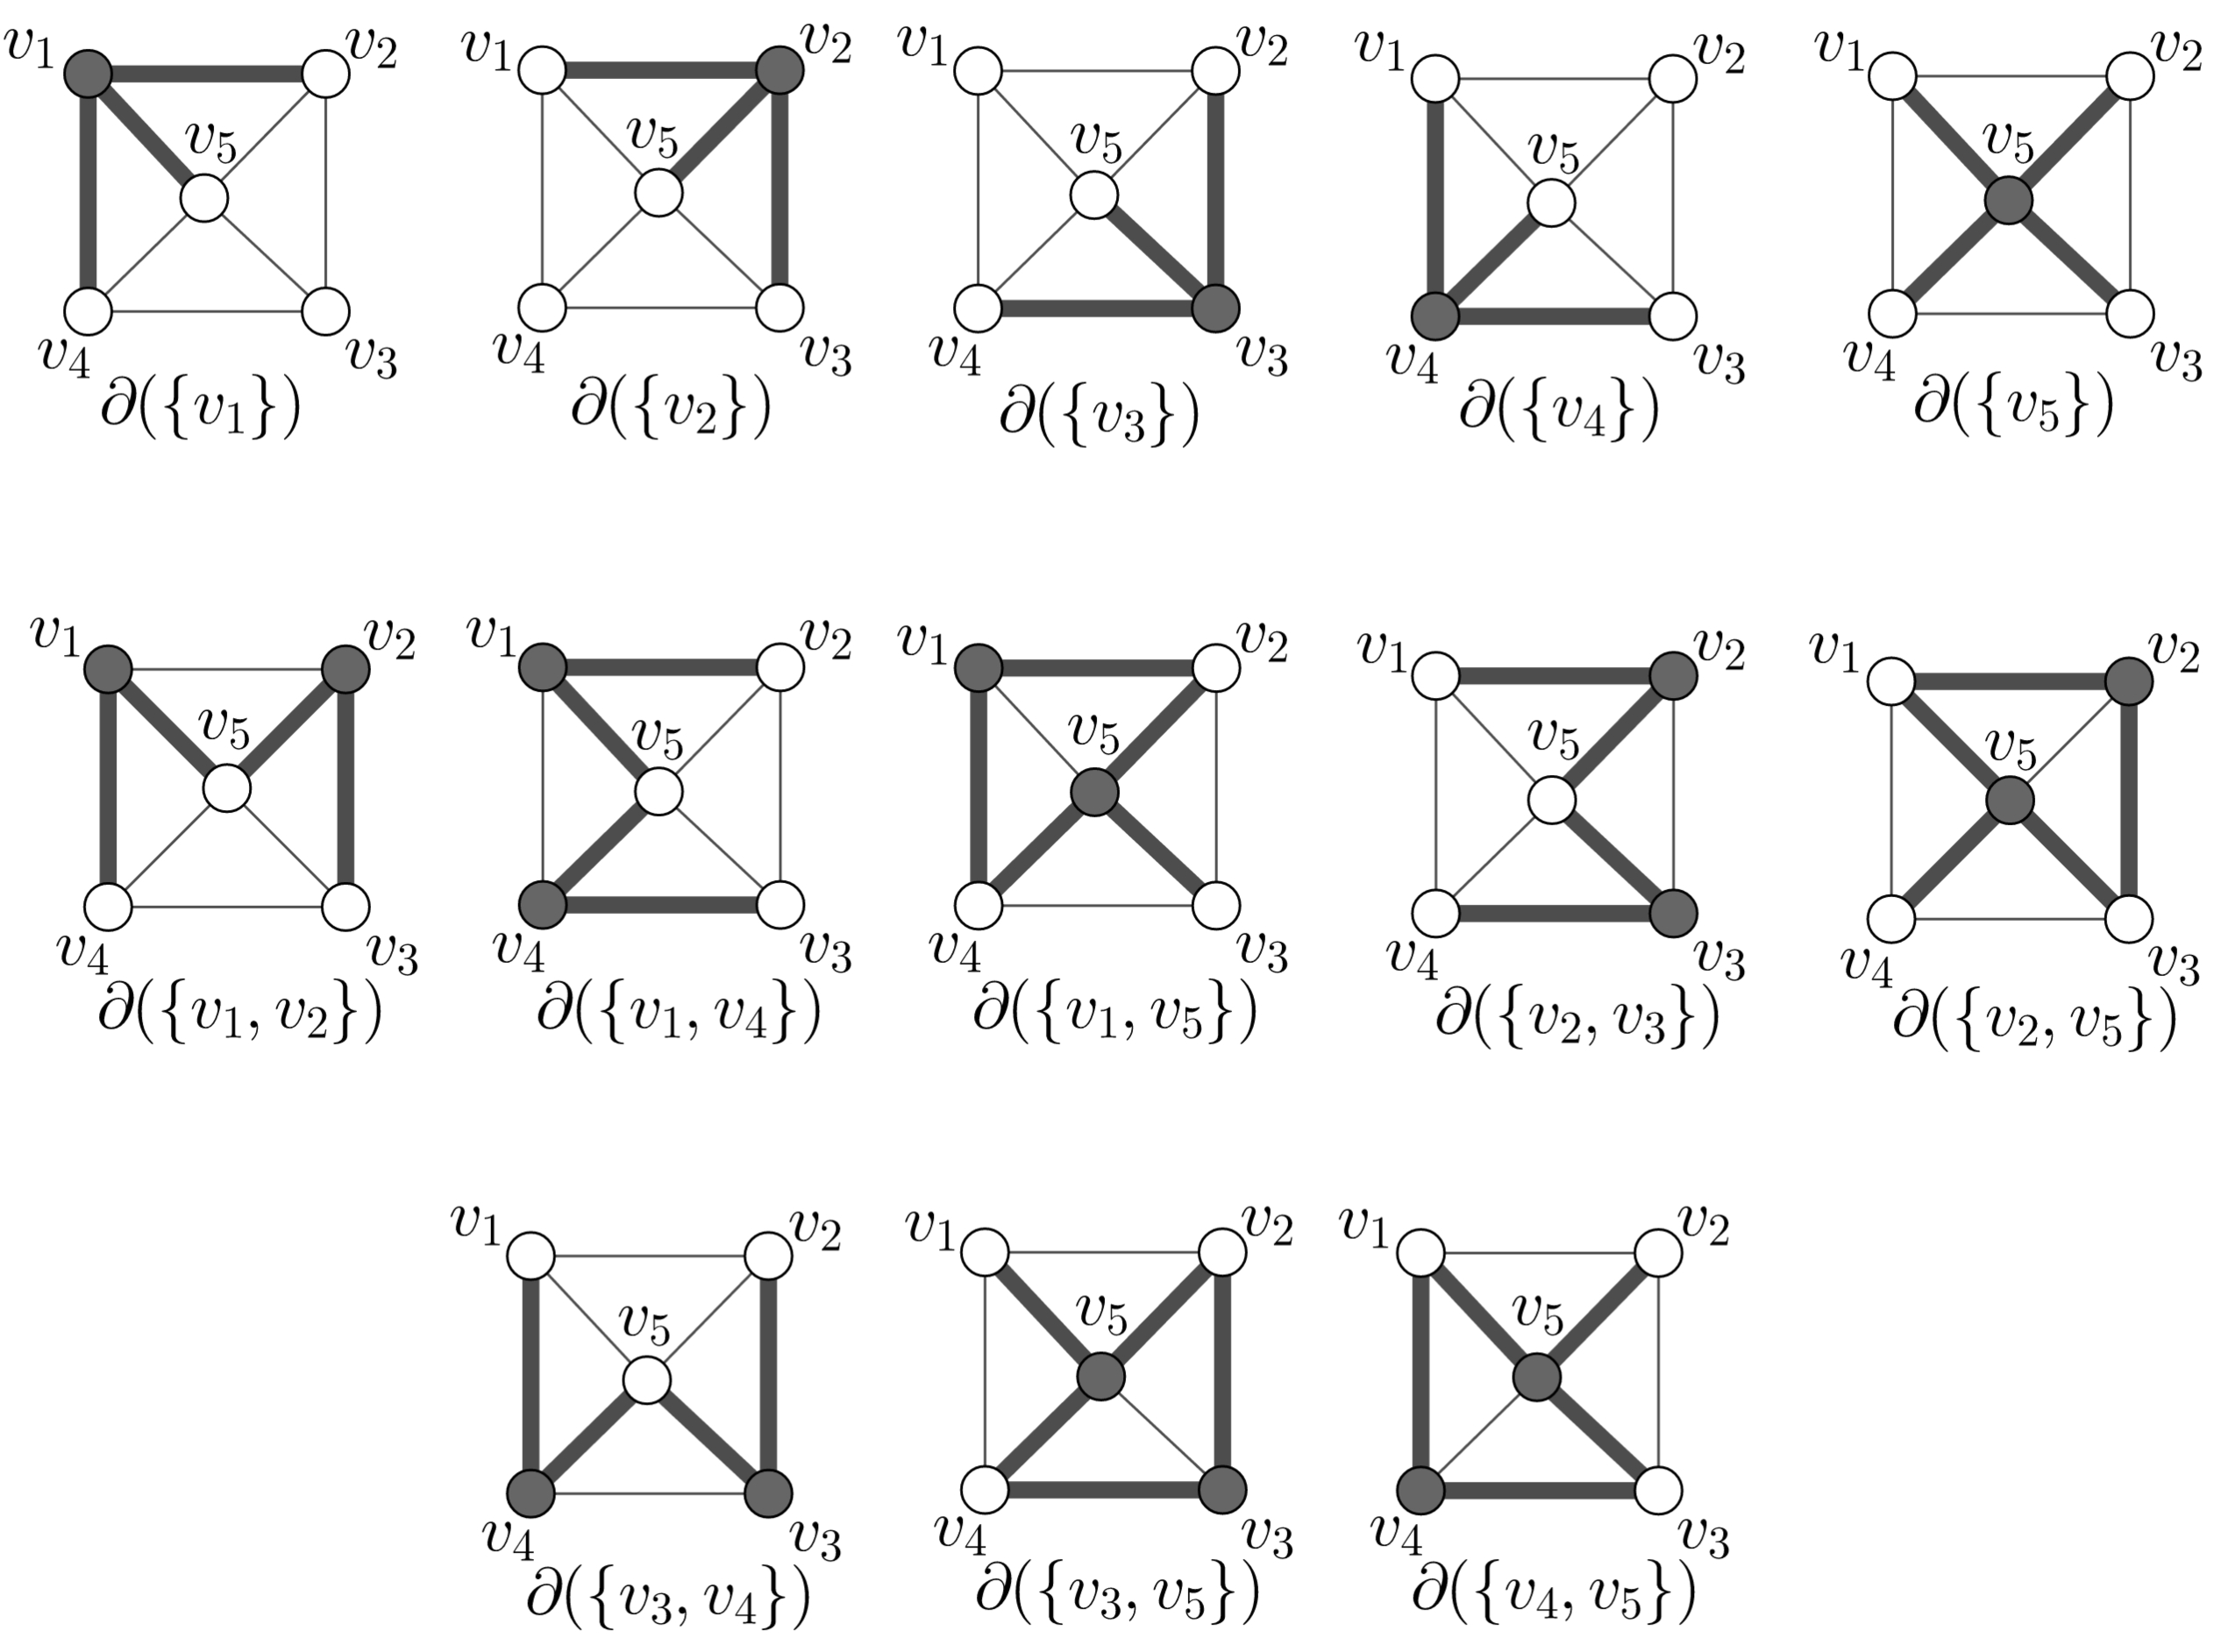
\includegraphics[scale=0.7]{img/imgchapter2/bond.jpg}
    \caption{Conjuntos de corte minimales de $W_{4}$}
    \label{fig:bondw4}
\end{figure}

\hfill $\blacklozenge$
\end{ejem}

Consideremos ahora una gráfica $G$ con $c$ componentes conexas, digamos $F_{1}, \ldots, F_{c}$. Supongamos que $X \subseteq V(G)$ es de tal manera que $\partial(X)$ es un conjunto de corte minimal de $G$. Si $X_{i} = X\cap V(F_{i})$, con $i \in \{1,\ldots,c \}$, anteriormente vimos que:
$$
    \partial_{G}(X) = \partial_{F_{1}}(X_{1}) \cup \cdots \cup \partial_{F_{c}}(X_{c}).
$$ 
Pero $\partial_{F_{i}}(X_{i}) = \partial_(X_{i})$ (porque no hay aristas entre diferentes componentes conexas), y la única diferencia es que $\partial_(X_{i})$ es un corte respecto a todo $G$ (y no sólo relativo a $F_{i}$). Por tanto, $\partial(X_{i}) \subseteq \partial(X)$, para todo $i\in \{1,\ldots, c\}$. 

Como $\partial(X)$ es minimal, entonces $\partial(X) = \partial(X_{j})$ (para aquellos $j\in\{1, \ldots, c\}$ tales que $\partial(X_{j}) \neq \emptyset$). Ésto sólo es posible (debido a la definición de $X_{j}$) si y sólo si, existe un único $k\in\{1, \ldots, c\}$, $X = X_{k}$.

Luego, $ \partial(X)= \partial(X_{k})$, es decir, $\partial(X)=\partial_{F_{k}}(X_{k})$. Concluimos estableciendo una proposición:
\begin{prop}\label{prop:cortesminimalesinconexa}
Los conjuntos de corte minimales de una gráfica inconexa son los conjuntos de corte minimales de sus componentes conexas. 
\end{prop}

La proposición previa nos ayudará a generalizar el corolario \ref{cor:corteminimalcomponentesconexas}:

\begin{teo} \label{teo:caracterizacionbond2}
Sea $G$ una gráfica. Si $X\subseteq V(G)$$, entonces $$\partial(X)$ es un corte minimal si y sólo si $$c(G\setminus \partial(X)) = c(G) + 1.$$
\end{teo}

\begin{proof}
Si $G$ es conexa, el teorema es válido por el corolario \ref{cor:corteminimalcomponentesconexas}.

Supongamos que $G$ es inconexa con $F_{1},\ldots,F_{c}$ sus componentes conexas y $c:=c(G)$. En primer lugar, supóngase que $\partial(X)$ es un conjunto de corte minimal de $G$. Por la proposición \ref{prop:cortesminimalesinconexa}, $\partial(X)$ es un corte minimal de alguna componente conexa $F_{j}$, es decir, $\partial(X) = \partial_{F_{j}}(X)$ y $X\subseteq V(F_{j})$. Entonces, de nuevo por el corolario \ref{cor:corteminimalcomponentesconexas},
$F_{k}\setminus \partial(X) = H_{1}\cup H_{2}$, donde $H_{1}$ y $H_{2}$ son sus componentes conexas. Por tanto, $$G\setminus \partial(X) = F_{1}\cup \cdots \cup F_{k-1}\cup H_{1} \cup H_{2}\cup F_{k+1}\cup\cdots \cup F_{c}.$$
De donde $c(G\setminus \partial(X)) = c(G) + 1$.

En segundo lugar, supóngase ahora que $c(G\setminus \partial(X)) = c(G) + 1.$ Si $G$ ya tenía $c$ componentes y ahora $G\setminus \partial(X)$ tiene una más, es imposible $\partial(X)$ tenga aristas de diferentes componentes conexas, porque a cada una la dividiría en al  menos dos partes y ya no habría $c+1$ componentes.

Por lo tanto, existe una componente $F_{k}$ tal que $\partial(X) \subseteq E(F_{k})$. Como $G\setminus \partial(X)$ tiene $c+1$ componentes conexas, necesariamente $F_{k}\setminus \partial(X)$ tiene dos componentes conexas. Ésto implica que $\partial(X)$ es un corte minimal de $F_{k}$. Por consiguiente, $\partial(X)$ es también un corte minimal de $G$, por la proposición \ref{prop:cortesminimalesinconexa}.

En conclusión, $\partial(X)$ es un corte minimal de $G$ si y sólo si $c(G\setminus \partial(X)) = c(G) + 1$.


\end{proof}
 

Si $B$ es un corte minimal contenido en un corte $\partial(X)$, de una gráfica $G$ conexa, ya sabemos (por el teorema anterior) que $G\setminus B = H_{1}\cup H_{2}$, donde $H_{1}$ y $H_{2}$ son sus componentes conexas. Es sencillo verificar que $B = \partial(Y)$, haciendo $Y:=V(F_{1})$. 

Por otro lado, como vimos en la demostración del teorema \ref{teo:caracterizacionbond2}, si $G$ es inconexa y $F_{1}, \ldots, F_{c}$ son sus componentes conexas, entonces $B$ es el corte minimal de alguna $F_{k}$. Digamos que $F_{k}\setminus B = H_{1}\cup H_{2}$, donde $H_{1}$ y $H_{2}$ son sus componentes conexas. Por lo que $G\setminus B =F_{1}\cup \cdots \cup F_{k-1}\cup H_{1} \cup H_{2}\cup F_{k+1}\cup\cdots \cup F_{c}$. Entonces, haciendo $Y:=V(H_{1})$, es claro que $B = \partial(Y)$.

Estos pequeños detalles se usan en la demostración del siguiente teorema que muestra la relación existente entre los conjuntos de corte minimales y aquellos que no lo son. 

\begin{teo}\label{teo:unionajenademinimales}
Sea $G$ una gráfica. Una subconjunto de $E(G)$ es un conjunto de corte de $G$ si y sólo si es es unión ajena de conjuntos de corte minimales de $G$.
\end{teo}

\begin{proof}
Para demostrar la necesidad, supongamos que $S \subseteq E(G)$ es un conjunto de corte. Si $S$ ya es minimal, terminamos. Si no, $S$ contiene a un conjunto de corte minimal, digamos $B_{1}$. Entonces, claramente, $S=B_{1} \cup (S \setminus B_{1})$. De nuevo, si $S \setminus B_{1}$ es un conjunto de corte minimal, terminamos. 

Si no es así, tomamos un minimal $B_{2} \subseteq (S \setminus B_{1})$ y observamos que $S=B_{1} \cup B_{2} \cup (S \setminus (B_{1} \cup B_{2}))$. Nos preguntamos si $S \setminus (B_{1} \cup B_{2})$ es minimal o no, y repetimos el mismo procedimiento anterior hasta terminar en un $q$-ésimo paso de tal forma que $B_{q} = S \setminus (B_{1} \cup \ldots \cup B_{q-1})$ sea un conjunto de corte minimal. Así, $S=B_{1} \cup \ldots \cup B_{q}$, y esta unión es ajena por construcción.

Para la suficiencia, asumimos ahora que $S=B_{1} \cup \ldots \cup B_{q}$ es unión ajena de conjuntos de corte minimales. Como cada $B_{i}$ es un corte, ya argumentamos, antes de enunciar este teorema,  que existe $Y_{i} \subseteq V(G)$ tal que $B_{i} = \partial(Y_{i})$. Luego, $S = \partial(Y_{1}) \cup \ldots \cup \partial(Y_{q})$. Sin embargo, la unión es ajena por hipótesis y, así, se tiene que $S=\partial(Y_{1}) \triangle \ldots \triangle \partial(Y_{q})$. Utilizando el teorema \ref{teo:diferenciasimetricacortes}, deducimos que $S=\partial(Y_{1} \triangle \ldots \triangle Y_{q})$. Por lo tanto, $S$ es un conjunto de corte.

Concluímos que $S \subseteq E(G)$ es un conjunto de corte si y sólo si es es unión ajena de conjuntos de corte minimales.  

\end{proof}


Sean $G$ una gráfica cualquiera y $X \subseteq V(G)$. El teorema anterior nos asegura la existencia de conjuntos de corte minimales (ajenos dos a dos) $B_{1},\ldots,B_{q} \subseteq E(G)$ tales que
$$\partial(X) = B_{1} \cup \cdots \cup B_{q}. $$
Entonces deducimos que las subgráficas generadoras correspondientes cumplen:
\begin{align*}
    G\Big[\partial(X)\Big] &= G [B_{1} \cup \cdots \cup B_{q}] \\
                           &= G [B_{1} \triangle \cdots \triangle B_{q}] \textnormal{ (la unión es ajena)}\\
                           &= G [B_{1}] \triangle \cdots \triangle G[B_{q}] \textnormal{ (por el corolario \ref{cor:difsimGeneradora})}.
\end{align*}

Luego, $G\Big[\partial(X)\Big]$ es una diferencia simétrica de subgráficas generadoras inducidas por cortes minimales. Nótese que no es una \textit{unión ajena de gráficas} pues, al ser generadoras, todas tienen el mismo conjunto de vértices, pero sí es una \textit{unión ajena por aristas} (recuerde que el teorema \ref{teo:unionajenademinimales} se refiere a una \textit{unión ajena} en el sentido conjuntista). Resumimos las ideas que acabamos de desarrollar en este corolario:

\begin{cor}\label{cor:unionajenademinimalesgeneradores}
Sea $G$ una gráfica. Una subgráfica generadora de $G$ inducida por un conjunto de corte puede expresarse como una diferencia simétrica de subgráficas generadoras de $G$ inducidas por conjuntos de corte minimales.
\end{cor}



\subsection{Conjuntos de corte fundamentales}
Los árboles generadores de una gráfica están relacionados de forma particular con los conjuntos de corte. Sea $T$ un árbol generador de $G$. Es común referirse a las aristas de $T$ como \textit{ramas}. Asimismo, llamamos \textit{coárbol} \index{Coárbol} al complemento de $T$ respecto a $G$, es decir, a la subgráfica generadora de $G$ cuyas aristas están determinadas por el conjunto $E(G)\setminus E(T)$. Lo denotamos como $\overline{T}$. 

\begin{prop}\label{prop:bondintersection}
Sean $T$ y $B$ un árbol generador y un conjunto de corte, respectivamente, ambos una gráfica $G$ conexa, tales que $B \neq  \emptyset$. Entonces siempre sucede que $\partial(X) \cap E(T) \neq \emptyset$.

\end{prop}

\begin{proof}
Supongamos que $B \cap E(T) = \emptyset$. Entonces $B \subseteq E(\overline{T})$ y, por tanto,\\ $E(T) = E(G)\setminus E(T) \subseteq E(G) \setminus B$. Así, $T$ es una subgráfica de $G\setminus B$. Sin embargo, $G\setminus B$ es inconexa y $T$ es un árbol generador  conexo, lo cual es una contradicción. Por lo tanto, $B \cap E(T) \neq \emptyset$ 

\end{proof}

La proposición anterior implica que  $\emptyset$ es el único conjunto de corte $G$ tal que  $\emptyset \subseteq \overline{T}$, es decir, que el corte vacío es el único conjunto de corte que está contenido en las aristas del coárbol $\overline{T}$.

Sea $b$ una rama cualquiera de $T$. Se sabe que $T \setminus b$ es inconexa y consta de dos componentes conexas: si no lo fuera, entonces en $T\setminus b$ habría una trayectoria $W$ que conecta los extremos de $b$. Entonces, en $T$, la trayectoria $W$ junto con la arista $b$ formaría un ciclo, lo cual es imposible; y consta de dos componentes porque sólo se retira una arista (que es adyacente a dos vértices).

Como $T \setminus b$ es inconexa, debe existir $X \subseteq V(T)=V(G)$ tal que $\partial_{T}(X) = \{b\}$. Entonces todas las aristas del corte $\partial_{G}(X)$ son elementos de  $E(\overline{T})\cup \{b\}$. Entonces $G\setminus \partial_{G}(X) = T \setminus b$. Lo anterior implica que la gráfica $G \setminus \partial_{G}(X)$ está constituida por dos componentes conexas, es decir, $\partial_{G}(X)$ es un corte minimal de $G$. 

Además, el corte $\partial_{G}(X)$ es único con la propiedad de estar contenido en $E(\overline{T})\cup \{b\}$. En efecto, digamos que hay otro corte de minimal $B$ tal que $B \subseteq E(\overline{T}) \cup \{b\}$. Luego,
\begin{align*}
(\partial_{G}(X) \triangle B) \cap E(T) &= (\partial_{G}(X) \cap E(T))\triangle(B\cap E(T))\\
&= \{b\} \triangle \{b\} \\
&= \emptyset.
\end{align*}
Entonces $\partial_{G}(X)\triangle B \subseteq E(\overline{T})$. Como el único conjunto de corte contenido en el coárbol es el vacío, entonces $\partial_{G}(X)\triangle B = \varnothing$, es decir, $\partial_{G}(X)=B$. Por tanto, $\partial_{G}(X)$ es el único corte con la propiedad de estar contenido en las aristas de $\overline{T}+b$.

\index{Conjunto de corte! fundamental}El corte $\partial_{G}(X)$ que construimos en los párrafos anteriores es llamado \textit{conjunto de corte fundamental de $G$ con respecto a $T$ y a $b$}, y lo denotaremos como $\mathscr{B}_{b}$ (quedando el árbol generador implícito). Es preciso mencionar que árboles generadores distintos darán lugar a cortes fundamentales distintos. Si $G$ tiene $n$ vértices, entonces sabemos (por el capítulo previo) que $T$ tiene $n-1$ ramas. Así,  necesariamente, $E(G)$ debe contener $n-1$ cortes fundamentales respecto a $T$.  

\begin{ejem} \label{ejem:cortesfundamentales}
\begin{figure}[H]
\vspace{-1.5cm}
    \centering
    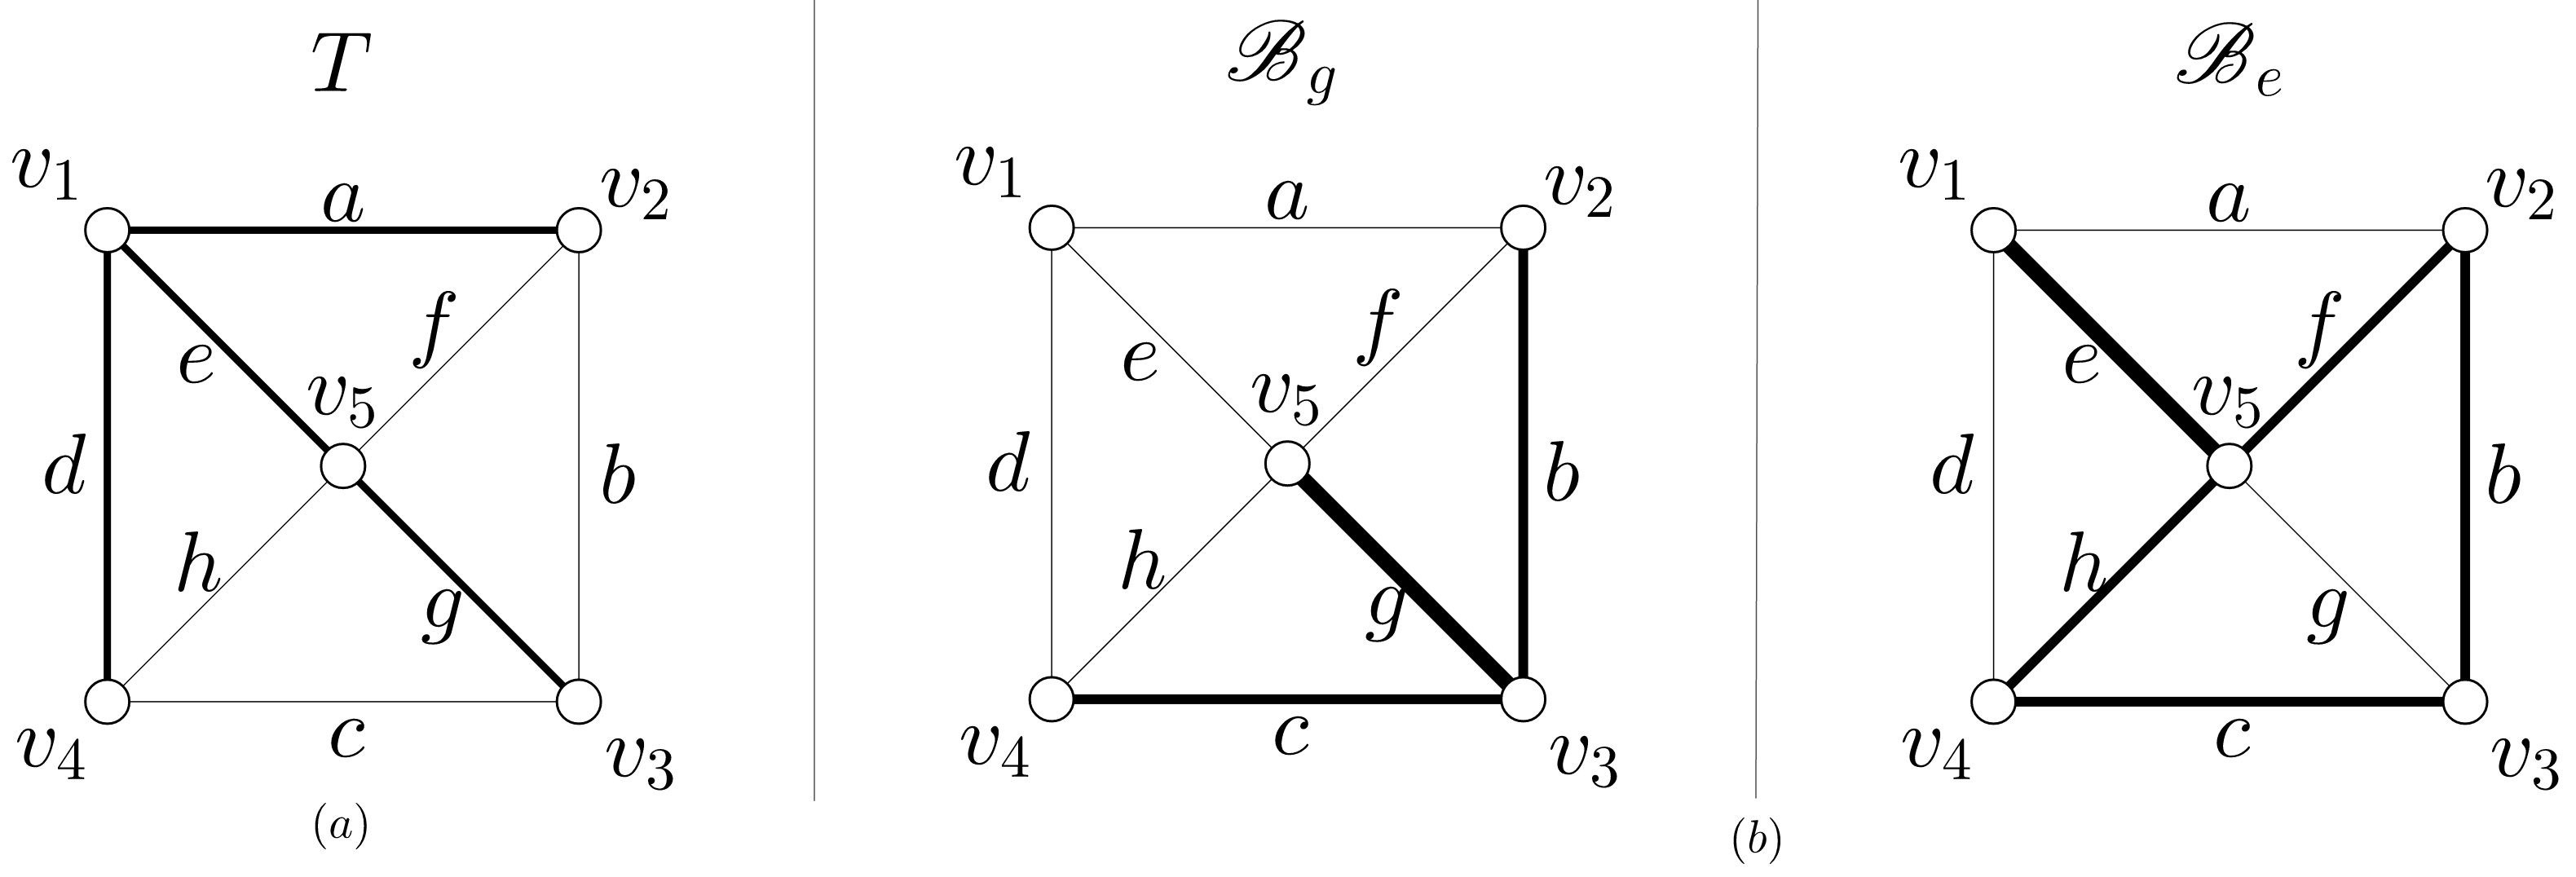
\includegraphics[scale = 0.18]{img/imgchapter2/bondminimales.jpg}
    \caption{}
    \label{fig:bondminimales}
\end{figure}


Recuérdese la gráfica rueda $W_{4}$ de la figura \ref{fig:wheel}. En la imagen \ref{fig:bondminimales}, en el inciso $(a)$, tomamos un árbol generador $T$ cuyas aristas son $\{a, d, e, g\}$. En el inciso $(b)$ mostramos dos cortes fundamentales, uno respecto a la rama $g$ y el otro respecto a $e$.


\hfill $\blacklozenge$
\end{ejem}



\begin{lema}\label{cortesfundamentalespropchida}
Sea $T$ un árbol generador de $G$ y $S\subseteq G$. Consideremos  
$$
B =\difsym_{b \in E(S)} \mathscr{B}_{b}. 
$$
Entonces $B$ es un conjunto de corte. Además, $B \cap E(T) = E(S)$ y $B$ es el único conjunto de corte de $G$ con esta propiedad.
\end{lema}

\begin{proof}
Que $B$ sea un conjunto de corte se da por el teorema \ref{teo:diferenciasimetricacortes}. Por otro lado,
\begin{align*}
    B \cap E(T) &=(\difsym_{b \in S} \mathscr{B}_{b}) \cap E(T) \\
             &=\difsym_{b \in S} (\mathscr{B}_{b} \cap E(T)) \\
             &=\difsym_{b\in S} \{b\} \\
             &= S.
\end{align*}
Además, si hubiese otro corte $B'$ tal que $B' \cap E(T)= S$, entonces $(B \triangle B') \cap E(T) = \emptyset$. Así, \\$B \triangle B' \subseteq E(\overline{T})$, implicando que $B \triangle B' = \emptyset$. Luego, $B = B'$, y $B$ es único.

\end{proof}

El lema anterior da pie al siguiente teorema, que caracteriza a los conjuntos de corte en términos de los cortes fundamentales.

\begin{teo} \label{teo:basecortesfundamentales}
Si $T$ es un árbol generador de $G$, entonces todo conjunto de corte de $G$ puede expresarse de manera única como una diferencia simétrica de conjuntos de corte fundamentales con respecto a $T$.
\end{teo}

\begin{proof}
Sea $\partial(X)$ un conjunto de corte cualquiera de $G$. Hacemos $S= \partial(X) \cap E(T)$. Por el teorema anterior, necesariamente, $\partial(X) = \difsym_{b \in S} \mathscr{B}_{b}$ y es el único con tales propiedades.

\end{proof}

En el caso que $G$ sea una gráfica inconexa, se toma un bosque generador maximal y la construcción de sus cortes fundamentales es análoga. Como los cortes fundamentales son, en particular, cortes minimales, entonces los cortes fundamentales de $G$ serán los cortes fundamentales de cada componente conexa; y los teoremas que hemos probado siguen siendo válidos para gráficas inconexas (con sus respectivas modificaciones). Si $G$ tiene $n$ aristas y $c$ componentes conexas, entonces sabemos que sus bosques generadores maximales tienen $n-c$ aristas; luego, $G$ tiene $n - c$ conjuntos de corte fundamentales. 

El teorema previo garantiza la \textit{unicidad} de la representación de los conjuntos de corte (lo que no aseguraba el teorema \ref{teo:unionajenademinimales}). Además, el teorema que acabamos de probar nos permite caracterizar de manera única a las subgráficas generadoras inducidas por conjuntos de corte (análogo al \ref{cor:unionajenademinimalesgeneradores}). Esta unicidad de la que hablamos será importante en el capítulo 3.

\begin{cor}\label{cor:DifSimUnicaDeFundamentales}
Sea $G$ una gráfica. Una subgráfica generadora de $G$ inducida por un conjunto de corte puede expresarse de manera única como una diferencia simétrica de subgráficas generadoras de $G$ inducidas por conjuntos de corte fundamentales.
\end{cor}






E\section{Gráficas pares de $G$}
Decimos que una gráfica es \textit{par} \index{Gráfica! par} si y sólo si todos sus vértices tienen grado par. En particular, los ciclos son gráficas pares pues todos sus vértices tienen grado $2$; así como la gráfica vacía $\varnothing$, cuyos vértices tienen grado $0$. Note que, si $H$ es una subgráfica par de $G$, la subgráfica generadora inducida $G[E(H)]$ es también par, pues sólo se están añadiendo vértices aislados. Entonces, en esta sección, basta con enfocarnos en estudiar las subgráficas pares de $G$. Primero probaremos algunos resultados que relacionan a los conjuntos de corte con las gráficas pares.  

\begin{lema} \label{lema1}
Sean $G$ una gráfica y $X \subseteq V(G)$. Entonces
$$
\big|\partial(X)\big|= \sum _{v \in X} d(v)- 2 \big |E[X]\big |.
$$
\end{lema}

\begin{proof} Para esta prueba haremos uso de la matriz de incidencia $\mathbf{M}_{G}$. Basándonos en las ideas que expusimos en el capítulo anterior, sabemos que se cumple:
\begin{equation} \label{eq4}
\sum_{v \in X} \sum_{e \in E(G)} m_{ve} = \sum_{e \in E(G)} \sum_{v \in X} m_{ve}.
\end{equation}

Se sabe también que $\sum_{e \in E(G)} m_{ve} = d(v)$, con $v \in X$. Así, en particular, 
\begin{equation} \label{eq5}
    \sum_{v \in X} \sum_{e \in E(G)} m_{ve} =\sum_{v \in X} d(v).
\end{equation}

Por otro lado, es sencillo darse cuenta que el conjunto de aristas se puede partir de la siguiente manera: $E(G)=\partial(X) \cup E[X] \cup E[\bar{X}]$. De aquí, dada una arista $e \in E(G)$, y de la definición de $\mathbf{M}_{G}$, se tiene
 $$
  \sum_{v \in X} m_{ve} = \left\{\begin{matrix}
1, & \text{si} \hspace{1.5mm} e \in \partial(X) \\ 
2, & \text{si} \hspace{1.5mm} e \in E[X]        \\
0, & \text{si} \hspace{1.5mm} e \in E[\bar{X}]
\end{matrix}\right.
 $$
 Luego, deducimos que:
  $$
  \sum_{e \in E(G)} \sum_{v \in X} m_{ve} = \sum_{e \in \partial(X)} \big( \sum_{v \in X} m_{ve} \big) + \sum_{e \in E[X]} \big(\sum_{v \in X} m_{ve}\big) + \sum_{e \in E[\bar{X}]} \big(\sum_{v \in X} m_{ve}\big).
  $$
  Por tanto, 
  \begin{equation} \label{eq6}
      \sum_{e \in E(G)} \sum_{v \in X} m_{ve} = \big| \partial(X) \big| + 2 \big| E[X] \big|.
  \end{equation}
  Sustituyendo las ecuaciones \ref{eq5} y \ref{eq6} en \ref{eq4}, y realizando las operaciones adecuacada, llegamos a la igualdad deseada: $\big|\partial(X)\big|= \sum _{v \in X} d(v)- 2 \big |E[X]\big |$.
  
  
\end{proof}




\begin{prop} \label{prop3}
$G$ es par si y sólo si $|\partial(X)|$ es par, para cualquier $X \subseteq V(G)$.
 
\end{prop}

\begin{proof}
Supongamos que $G$ es par y sea $X$ un subconjunto de vértices de $G$. De la paridad de $G$ se deduce que $\sum_{v \in X} d(v)$ es par. Luego entonces $\sum _{v \in X} d(v)- 2 \big |E[X]\big |$ es par y, por el lema \ref{lema1}, $\big|\partial(X)\big|$ también es par.

En segundo lugar, asumimos que $\big|\partial(X)\big|$ es par, con $X$ cualquier subconjunto de vértices de $G$. En particular, dado $v \in V(G)$, $\big|\partial(\{v\})\big|$ es par. En la sección pasada mencionamos que en $\partial(\{v\})$ se encuentran todas las aristas que inciden en $v$, excepto sus posibles lazos. Si $\partial(\{v\}) = \emptyset$ y $v$ no tiene lazos, entonces su grado es cero. Si $v$ tiene lazos, recordemos que estos se cuentan doble para el grado, de forma que éste sería par de todos modos. Si, ahora, $\partial(\{v\}) \neq \emptyset$, como $\big| \partial(\{v\}) \big|$ es par, inciden en $v$ un cantidad par de aristas y, si tuviera lazos, éstos se cuentan doble, de tal manera que $d(v)$ es un número par. Por lo tanto, todos los vértices de $G$ tienen grado par, i.e., $G$ es par.

Luego, $G$ es par si y sólo si, para todo $X \subseteq V(G)$, $|\partial(X)|$ es par.

\end{proof}

Para la demostración del siguiente teorema es necesario recordar que $|A \triangle B| = |A|+|B| - 2|A \cap B|$.

\begin{teo} \label{teo:difsimciclos}
 Dada $G$ una gráfica, la diferencia simétrica de dos subgráficas pares de $G$ es también una subgráfica par de $G$.
\end{teo}

\begin{proof}
Sean $C_{1}, C_{2}$ dos subgráficas pares cualesquiera de $G$. Tomamos un subconjunto $X$ de vértices de $G$. Por la proposición \ref{prop2}, es cierto que 
$$\partial_{C_{1} \triangle C_{2}}(X) = \partial_{C_{1}}(X) \triangle \partial_{C_{2}}(X).$$
Además, en virtud de la proposición \ref{prop3}, $|\partial_{C_{1}}(X)|$ y $|\partial_{C_{2}}(X)|$ son números pares. Entonces 
$$|\partial_{C_{1}}(X) \triangle \partial_{C_{2}}(X)| = |\partial_{C_{1}}(X)| + |\partial_{C_{2}}(X)| - 2 |\partial_{C_{1}}(X) \cap \partial_{C_{2}}(X)|$$
es también un número par, es decir, $\partial_{C_{1} \triangle C_{2}}(X)$ tiene cardinalidad par. De nuevo por la proposición \ref{prop3}, concluímos que $C_{1} \triangle C_{2}$ es una subgráfica par.

\end{proof}

Utilizando el Principio de Inducción, es claro que el teorema anterior puede generalizarse a cualquier cantidad arbitraria de subgráficas pares.

\subsection{Los ciclos de $G$}
Por simplicidad, a partir de aquí, cuando digamos \textit{ciclos ajenos} nos referiremos a ciclos \textit{ajenos por aristas}. También introducimos un nuevo concepto: una \textit{descomposición de una gráfica $G$} \index{Descomposición de una gráfica} es una familia $\mathcal{F}$ de subgráficas ajenas por aristas tales que:
$$
\bigcup_{F \in \mathcal{F}} E(F) = E(G).
$$
En \cite{Bondy,Seshu,Deo, Biggs} se mencionar que a principios del siglo XX, Oswald Veblen (1880 - 1960) caracterizó las gráficas pares como aquellas que pueden ser descompuestas en ciclos ajenos. A continuación presentamos dicho resultado y su justificación.

\begin{teo}[\textit{\textbf{Teorema de Veblen}}] \label{teo:veblen}
Una gráfica $G$ es par si y sólo si $G$ se descompone en ciclos ajenos.
\end{teo}

\begin{proof}
Probemos la \textit{necesidad} por inducción fuerte, sobre el número $m$ de aristas de $G$. 

\underline{Paso base}: $m=0$. Entonces $G$ no tiene aristas, i.e., es una gráfica vacía (que es par) y se descompone en una familia vacía de ciclos.

\underline{Hipótesis de inducción}: Supongamos que, para cualquier gráfica par $H$ con $q$ aristas y $q < m$, $H$ admite una descomposición en ciclos ajenos.

\underline{Paso inductivo}: Sea $G$ una gráfica par con $m$ aristas. Tomamos $F$ la subgráfica de $G$ inducida por sus vértices de grado positivo (en otras palabras, ignoramos, de momento, los posibles vértices aislados de $G$). Dado un vértice $v \in V(F)$, por la paridad de $G$, sabemos que $d_{F}(v)\geq 2$; y, por el teorema \ref{teo:ciclos}, necesariamente $F$ contiene un ciclo, digamos $C$. Es claro también que $C$ está contenido en $G$.

Consideramos a $H = G \setminus E(C)$. Verifiquemos que esta gráfica, en efecto, es par. Tomamos $v$ un vértice cualquiera de $H$. Como $V(H) = V(G)$, entonces $v \in V(G)$. Si es un vértice aislado, entonces su grado es par. Si no es aislado, entonces hay dos posibilidades: que $v$ sea parte del ciclo $C$ o no. Si $v \in V(C)$, significa que hay dos aristas de $C$ que inciden en él. Entonces, en $H$, se remueven tales aristas, disminuyendo en dos el grado de $v$ (conservando así la paridad). Si $v \notin V(C)$, su grado permanece invariante en $H$. En cualquier caso, debido a que $G$ es par, el grado de $v$ es un número par. 

Podemos resumir las ideas anteriores en la siguiente ecuación:
$$
  d_{H}(v) = \left\{\begin{matrix}
0, & \text{si} \hspace{1.5mm} d_{G}(v)=0 \\ 
d_{G}(v)-2, & \text{si} \hspace{1.5mm} v \in V(C)     \\
d_{G}(v), & \text{si} \hspace{1.5mm} v \notin V(C)
\end{matrix}\right..
$$
Por lo tanto, $H$ es una gráfica par con menos aristas que $G$. Gracias a la hipótesis de inducción sabemos que $H$ se descompone en una familia $\Gamma$ de ciclos ajenos, es decir:
$$
E(H) = \bigcup_{\gamma \in \Gamma} E(\gamma).
$$

Dada la igualdad anterior, y como $H = G\setminus E(C)$, entonces $C$ es un ciclo ajeno respecto a los ciclos que pertenecen a $\Gamma$. Por lo tanto, 
$$
E(G) = E(H) \cup E(C) = \big( \bigcup_{\gamma \in \Gamma} E(\gamma) \big) \cup E(C). 
$$
Por consiguiente, $G$ se descompone en la familia de ciclos ajenos $\Gamma \cup \{C\}$. Por inducción, concluimos que cualquier gráfica par puede ser descompuesta en ciclos ajenos.

Probaremos ahora la \textit{suficiencia}. Supongamos que $G$ admite una descomposición en ciclos, es decir, que existen $\gamma_{1}, \ldots, \gamma_{q}$ ciclos ajenos contenidos en $G$ tales que 
$$
\bigcup_{i=1}^{q} E(\gamma_{i}) = E(G).
$$

Sea $v$ un vértice cualquiera de $G$. Si $v$ es aislado, o sea $d_{G}(v)=0$, entonces tiene grado par. Si $d_{G}(v)\neq 0$, significa que hay al menos otro vértice $u$ adyacente a $v$. Supongamos que $a$ es la arista cuyos extremos son $u$ y $v$. Como $a \in \bigcup_{i=1}^{q} E(\gamma_{i})$, existe un ciclo $\gamma_{j}$ tal que $a \in E(\gamma_{j})$, esto es, que $v$ es un vértice del ciclo $\gamma_{j}$, lo cual implica que existe otro vértice $w$ (éste puede ser el mismo $v$ o, incluso, $u$) adyacente a $v$. En resumen, por cada ciclo al que pertenezca $v$ otros dos vértices (no necesariamente distintos) son adyacentes a $v$, de donde $d_{\gamma_{j}}(v) = 2$. 

Por otro lado, es fácil observar que el grado de cada vértice de $G$ es la suma de los grados de ese mismo vértice respecto a cada subgráfica de la descomposición. Luego, suponiendo que $v$ es vértice de $p$ ciclos (digamos $\gamma_{j_{1}}, \ldots, \gamma_{j_{p}}$) en la descomposición, el párrafo anterior nos permite afirmar que

$$
d_{G}(v) = \sum_{i=1}^{p}d_{\gamma_{j_{i}}}(v)=\sum_{i=1}^{p}2=2p.
$$

Así, el grado de todo vértice de $G$ es el doble del número de ciclos a los que pertenece y, en consecuencia, $G$ es una gráfica par. 

Por lo tanto, $G$ es par si y sólo si $G$ se descompone en ciclos ajenos.

\end{proof}


En el Teorema de Veblen, la descomposición en ciclos ajenos puede interpretarse como una diferencia simétrica de ciclos ajenos por aristas. Aún más, podemos generalizarlo en el siguiente corolario:

\begin{cor}\label{teo:veblen2}
Dada una gráfica $G$, toda subgráfica generadora de $G$ es par si y sólo si es una diferencia simétrica de subgráficas generadoras inducidas por ciclos ajenos de $G$.
 \end{cor}
 
 \begin{ejem}
\begin{figure}[H]
\vspace{-0.55cm}
    \centering
    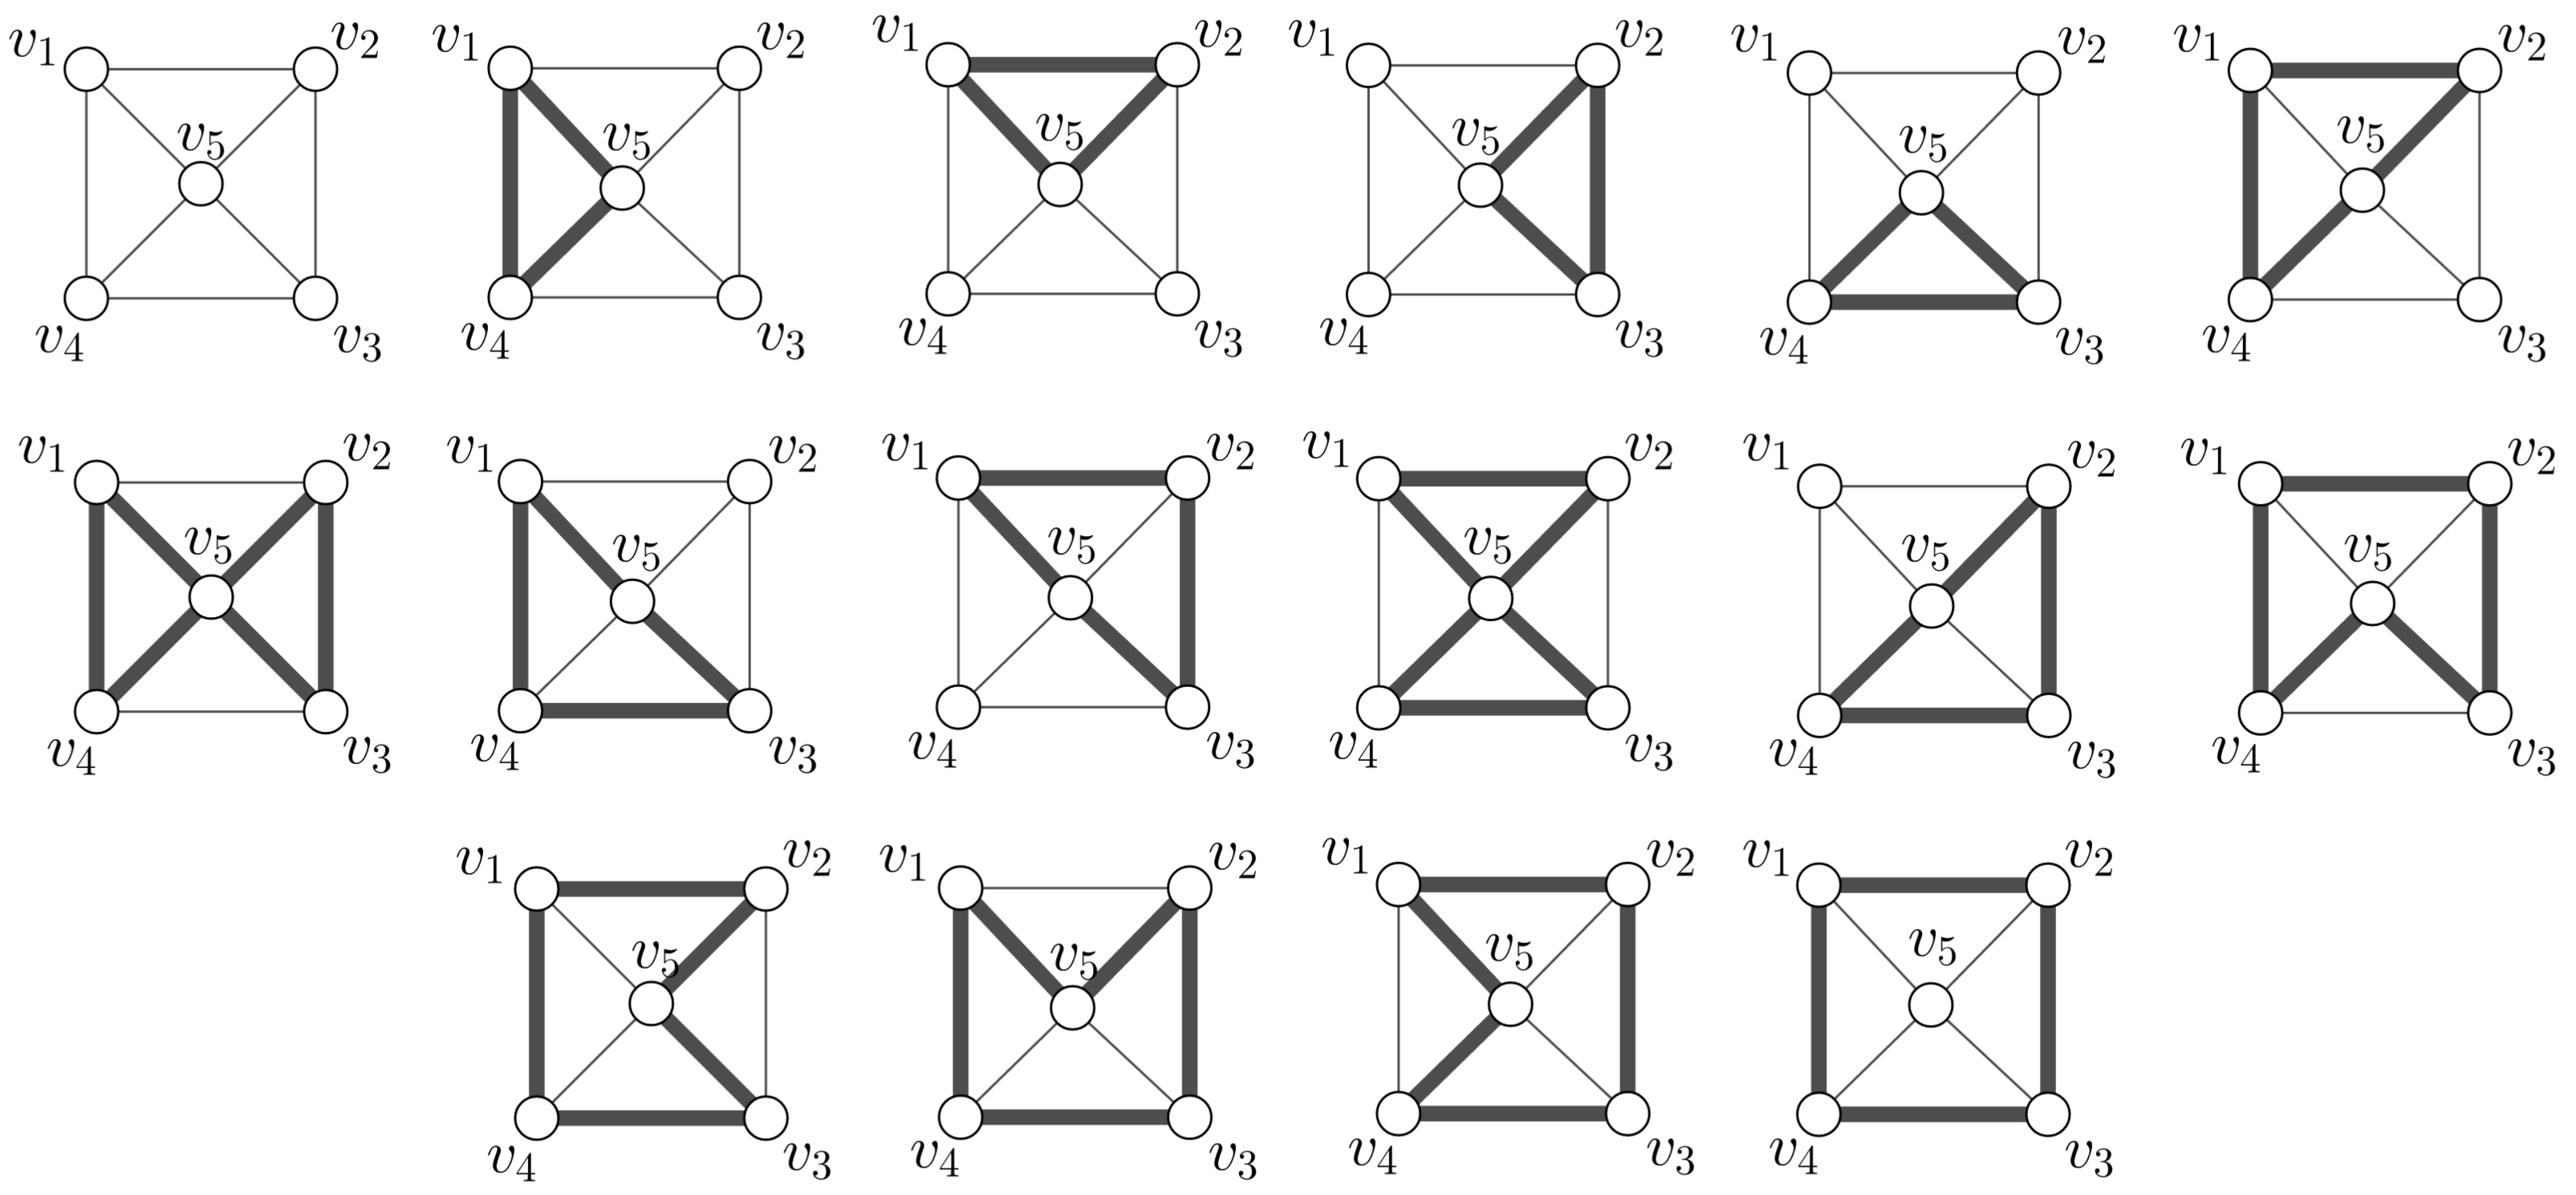
\includegraphics[scale=0.6]{img/imgchapter2/Espaciodeciclos.jpg}
    \caption{}
    \label{fig:espaciociclos}
\end{figure}
En la figura \ref{fig:espaciociclos} se encuentran todas las subgráficas pares de la gráfica $W_{4}$ y hemos resaltado sus respectivas aristas. El lector podrá darse cuenta cómo cada subgráfica par de $W_{4}$ o es un ciclo o puede ser descompuesto en ciclos ajenos.

\hfill $\blacklozenge$
\end{ejem}


\subsection{Ciclos fundamentales}
Los ciclos están especialmente relacionados con los complementos de árboles generadores, como veremos a continuación.

\begin{prop}
Sean una subgráfica generadora par $H$ de $G$, distinta de la subgráfica vacía $\varnothing$, y un árbol generador $T$. Entonces $H \cap \overline{T} \neq \varnothing$.
\end{prop}

\begin{proof}
Para llegar a una contradicción, supongamos que $H \cap \overline{T} = \varnothing$, entonces \\$E(H) \cap E(\overline{T}) = \emptyset$. Luego, $E(H) \subseteq E(T)$ y, de este modo, $H$ es una subgráfica de $T$

Por el corolario del teorema de Veblen, $H$ se descompone en subgráficas generadoras inducidas por los ciclos de $G$. Entonces $T$ contiene estos ciclos. Sin embargo, esto es una contradicción pues $T$ es un árbol. 
Por tanto, $C \cap \overline{T} \neq \varnothing$.

\end{proof}

De este resultado se desprende que la única subgráfica par contenida en $T$ es la subgráfica vacía $\varnothing$. Ahora tomemos una arista $c$ cualquiera  de $\overline{T}$ y supongamos que $x$ y $y$ son sus extremos. De la proposición \ref{prop:treepath}, sabemos que hay una única trayectoria $P$, contenida en $T$, que une a $x$ y a $y$. 

Por tanto, la gráfica $T + c$ contiene al ciclo formado por la trayectoria $P$ y la arista $c$, llamado \index{Ciclo! fundamental}\textit{ciclo fundamental de $G$ con respecto a $T$ y a $c$}. Téngase en cuenta que diferentes árboles generadores determinan ciclos fundamentales distintos. Cuando esté implícito el árbol con el que estemos trabajando, escribiremos como $\mathscr{C}_{c}$ a la subgráfica generadora inducida por el ciclo fundamental con respecto a $c$ (y, por comodidad, esta subgráfica también será llamada \textit{ciclo fundamental}). Si $G$ es inconexa, sus ciclos fundamentales, con respecto a algún bosque generador maximal, son los ciclos fundamentales de cada componente conexa. 

Sabemos que hay $m - n + 1$ aristas en $\overline{T}$, entonces $G$ debe contener $m - n +1$ ciclos fundamentales con respecto a $T$.  Por último, si $G$ tiene $c$ componentes conexas y, puesto que hay $m - n + c$ aristas en el complemento de cualquier bosque generador maximal, necesariamente $G$ tiene $m-n+c$ ciclos fundamentales.

De forma análoga al comportamiento de los cortes fundamentales, la diferencia simétrica de dos ciclos fundamentales es una gráfica par (por el teorema \ref{teo:difsimciclos}). Además, por construcción, es claro que $E(\mathscr{C}_{c}) \cap E(\overline{T}) = \{c\}$ y que $\mathscr{C}_{c}$ es una subgráfica de $T + c$. De hecho, el siguiente teorema hace uso de estas dos observaciones.

\begin{lema} \label{ciclosfundamentalespropchida}
Sean $S$ una subgráfica generadora de una gráfica $G$ y $\overline{T}$ un coárbol de $G$. Supongamos que $S$ es una subgráfica de $\overline{T}$ y consideremos  
$$
H =\difsym_{c \in E(S)} \mathscr{C}_{c} 
$$
 Entonces $H$ es una subgráfica par. Además, $H \cap \overline{T} = S$ y $H$ es la única subgráfica par de $G$ con esta propiedad.
\end{lema}
 
 \begin{proof}
 Que $H$ sea par se da por el teorema \ref{teo:difsimciclos}. Por otro lado, nótese que
\begin{align*}
    H \cap \overline{T} &=(\difsym_{c \in E(S)} \mathscr{C}_{c}) \cap \overline{T} \\
             &=\difsym_{c \in E(S)} (\mathscr{C}_{c} \cap T) \\
             &=G\Big[\difsym_{c\in E(S)} c\Big] \\
             &= S.
\end{align*}
Además, si hubiese otra subgráfica par $H'$ tal que $H' \cap \overline{T}= S$, entonces $(H \triangle H') \cap \overline{T} = \varnothing$. Ésto, como se mencionó previamente, implica que  $H\triangle H' $ está contenida $T$. Pero eso significa que $H\triangle H' = \varnothing$ y, por tanto, $H = H'$. Luego, $H$ es única.
 \end{proof}

Hallamos en el lema previo hay una garantía de \textit{unicidad} en la representación de las subgráficas pares (y esto no lo aseguraba el Teorema de Veblen). Esta unicidad también será importante en el capítulo 3. Podemos generalizar lo anterior (en términos de subgráficas generadoras): 

 \begin{teo} \label{cor:baseciclosfundamentales}
Sean $G$ una gráfica y $T$ un árbol generador.Entonces toda subgráfica par de $G$ puede expresarse de manera única como una diferencia simétrica de subgráficas generadoras inducidas por los ciclos fundamentales con respecto a $T$  
 \end{teo}
 
 \begin{proof}
 Sea $H$ una subgráfica par cualquiera de $G$. Hacemos $S= H \cap \overline{T}$. Por el lema anterior, necesariamente, $H = \difsym_{c \in E(S)} \mathscr{C}_{c}$ y es el único con tales propiedades. 
 
 \end{proof}
 
 
 \begin{ejem}
 Recuérdese el ejemplo \ref{ejem:cortesfundamentales} y el árbol generador $T$ que habíamos escogido para $W_{4}$ (que vemos remarcado en el inciso $(a)$ de la imagen \ref{fig:ciclosfundamentales}). En el inciso $(b)$ mostramos dos ciclos fundamentales, uno respecto a la arista $h$ y el otro respecto a $b$.
 
 \begin{figure}[H]
     \centering
     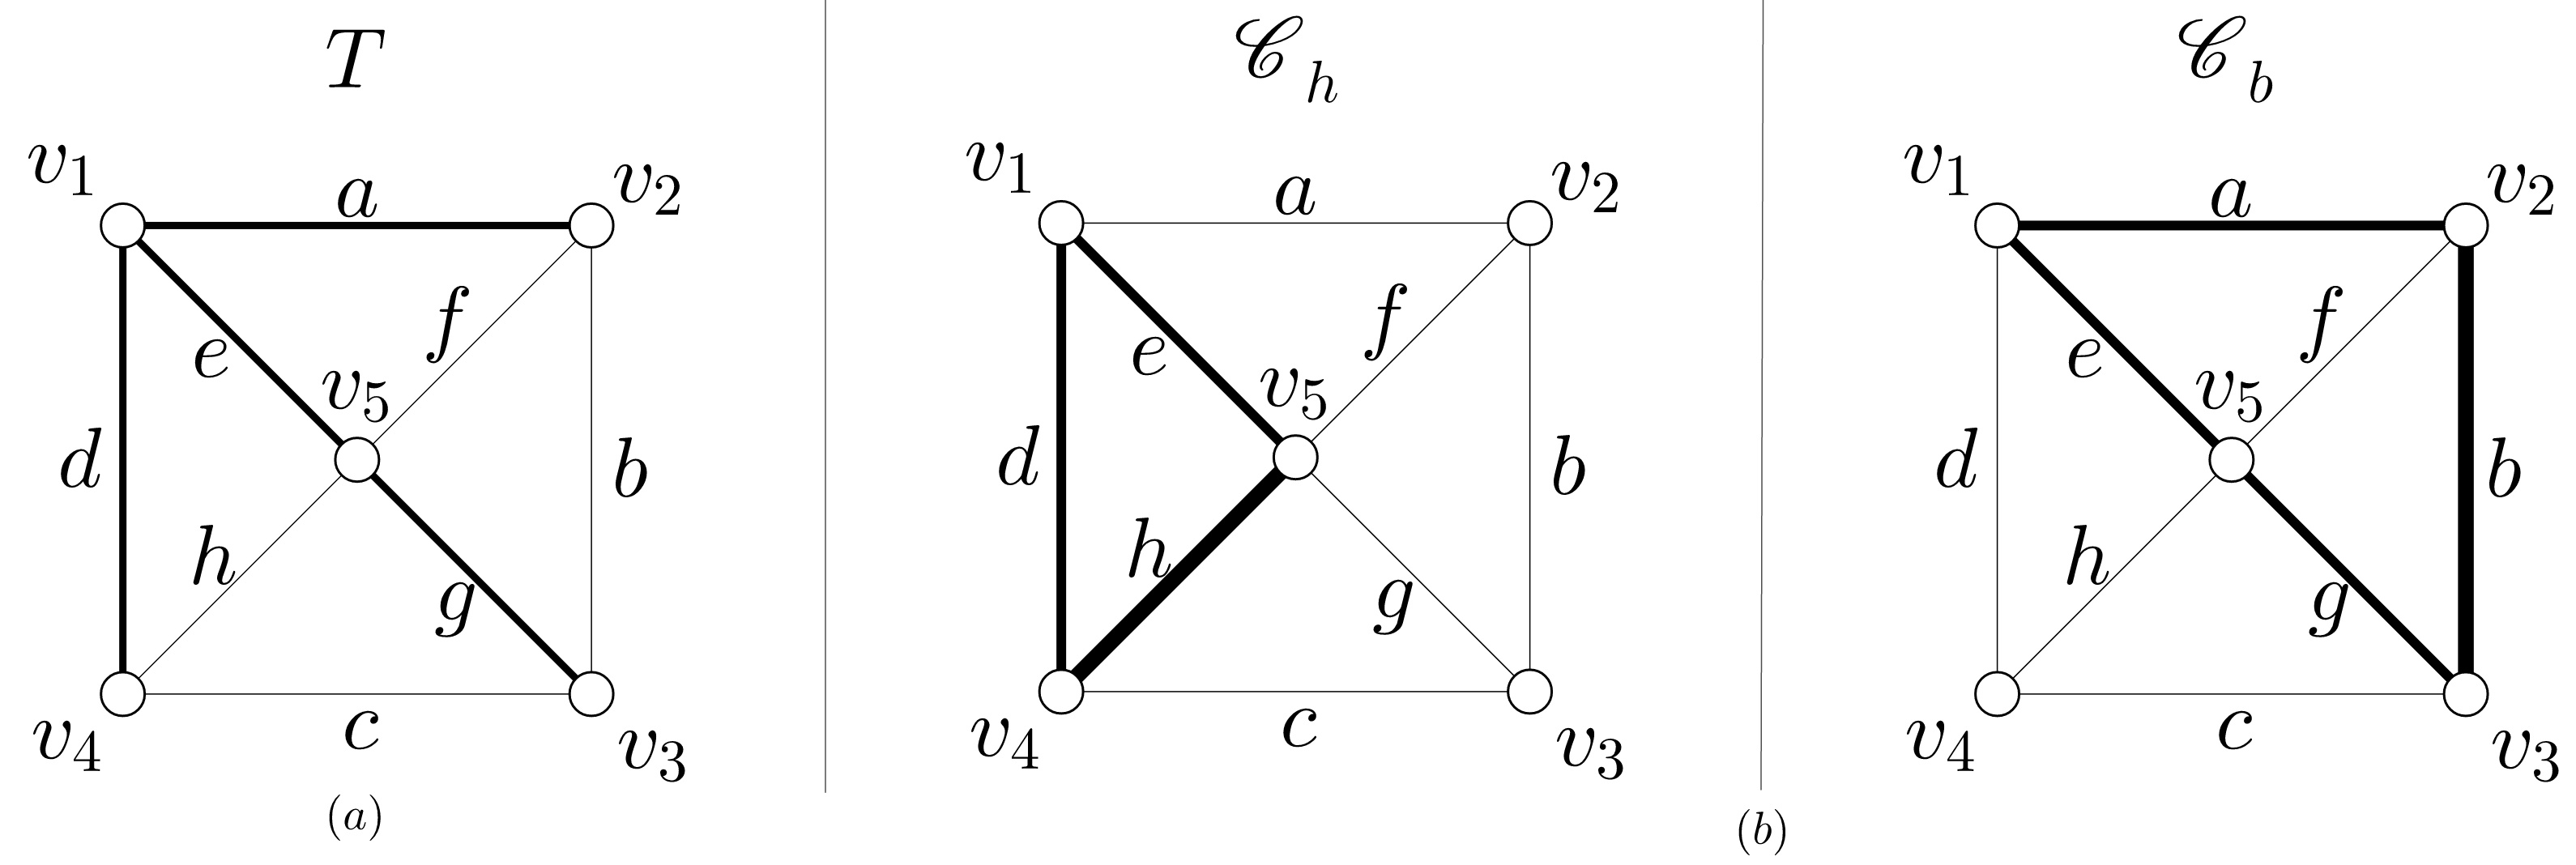
\includegraphics[scale=0.15]{img/imgchapter2/ciclosfundamentales.jpg}
     \caption{}
     \label{fig:ciclosfundamentales}
 \end{figure}
 
 \hfill $\blacklozenge$.
 \end{ejem}
 
 \section{Relación entre los conjuntos de corte y las gráficas pares}
 Sea $G$ una gráfica y tomemos un ciclo $C$ de $G$ y un vértice $u\in V(G)$. Es sencillo convencerse de que $\partial(u) \cap E(C)$ sólo tiene dos posibilidades: ser vacío o tener dos aristas como únicos elementos. En efecto, si $u$ no está en el ciclo $C$, no hay aristas en $\partial(u) \cap E(C)$; y si $u$ es parte del ciclo $C$, forzosamente dos aristas de $\partial(u)$ están en $C$ (si hubiera más, $C$ ya no sería un ciclo).  En ambos casos, tal intersección es de cardinalidad par. De hecho, generalizamos estas observaciones en el siguiente teorema.

\begin{teo} \label{teo:interseccionpar}
En cualquier gráfica, toda subgráfica par y todo conjunto de corte, tienen en común una cantidad par de aristas.
\end{teo}

\begin{proof} Sean $G$ una gráfica y $\partial(X)$ un conjunto de corte cualquiera, con $X \subseteq V(G)$. Si este corte es vacío, el teorema se cumple. 

Supongamos que $\partial(X) \neq \emptyset$. Probemos el teorema primero para ciclos y luego para gráficas pares en general. Recordemos que $G\setminus \partial(X) = G[X] \cup G[\overline{X}]$.

Sea $C$ un ciclo de $G$. Si este ciclo está completamente contenido en $G[X]$ ó $G[\overline{X}]$, también el teorema se cumple pues $E(C) \cap \partial(X) = \emptyset$.

La otra posibilidad es que $E(C) \cap \partial(X) \neq \emptyset$. Si ésto ocurre, significa que existe una arista con un extremo en $X$ y otro en $\overline{X}$. De tal manera que, partiendo del extremo en $X$, el ciclo atraviesa la gráfica hasta regresar al vértice donde empezó. Entonces $C$ cruza de $X$ a $\overline{X}$ las mismas veces que cruza de $\overline{X}$ a $X$. Por tanto, en ambos casos, $|C \cap \partial(X)|$ es un número par .

Ahora, sea $H$ una gráfica par. Gracias al teorema teorema de Veblen, sabemos que existen $C_{1},\ldots, C_{k}$ ciclos ajenos tales que $\bigcup_{j=1}^{k}C_{j} = H$. Entonces  
\begin{align*}
    |E(H) \cap \partial(X)| &= |(\bigcup_{j=1}^{k}E(C_{j})) \cap \partial(X)|\\
                      &= |\bigcup_{j=1}^{k} (E(C_{j}) \cap \partial(X))|.\\
\end{align*}
Como los ciclos $C_{i}$ son ajenos, también las intersecciones $E(C_{j}) \cap \partial(X)$. Luego, 
\begin{align*}
    |\bigcup_{j=1}^{k} (E(C_{j}) \cap \partial(X))| &= \sum_{j=1}^{k} |E(C_{j}) \cap \partial(X)|.
\end{align*}
Ya argumentamos al principio de esta prueba que los sumandos $|E(C_{j}) \cap \partial(X)|$ son pares, por lo tanto, su suma es par. Dado que $
    \sum_{j=1}^{k} |E(C_{j}) \cap \partial(X)| =  |E(H) \cap \partial(X)| $, entonces $ |E(H) \cap \partial(X)|$ es par, es decir, hay una cantidad par de aristas en $E(H) \cap \partial(X)$.
    
\end{proof}

¿Hay conjuntos de corte que son gráficas pares también? ¿O son conceptos mutuamente excluyentes? La respuesta es afirmativa: hay gráficas pares que, al mismo tiempo, son conjuntos de corte, como vemos en el siguiente ejemplo.
\vspace{0.5cm}
\begin{ejem} \label{ejem:k4ciclocorte}
Consideremos a $K_{4}$, la gráfica completa de cuatro vértices (inciso $(a)$ de la figura \ref{fig:k4ciclocorte}). Es evidente que contiene al ciclo $C_{4}$, cuyas aristas son $\{a,b,c,d\}$. Si observamos atentamente, uno puede darse cuenta que $\partial{\{u_{1},u_{3}\}} = E(C_{4})$.

 \begin{figure}[H]
     \centering
     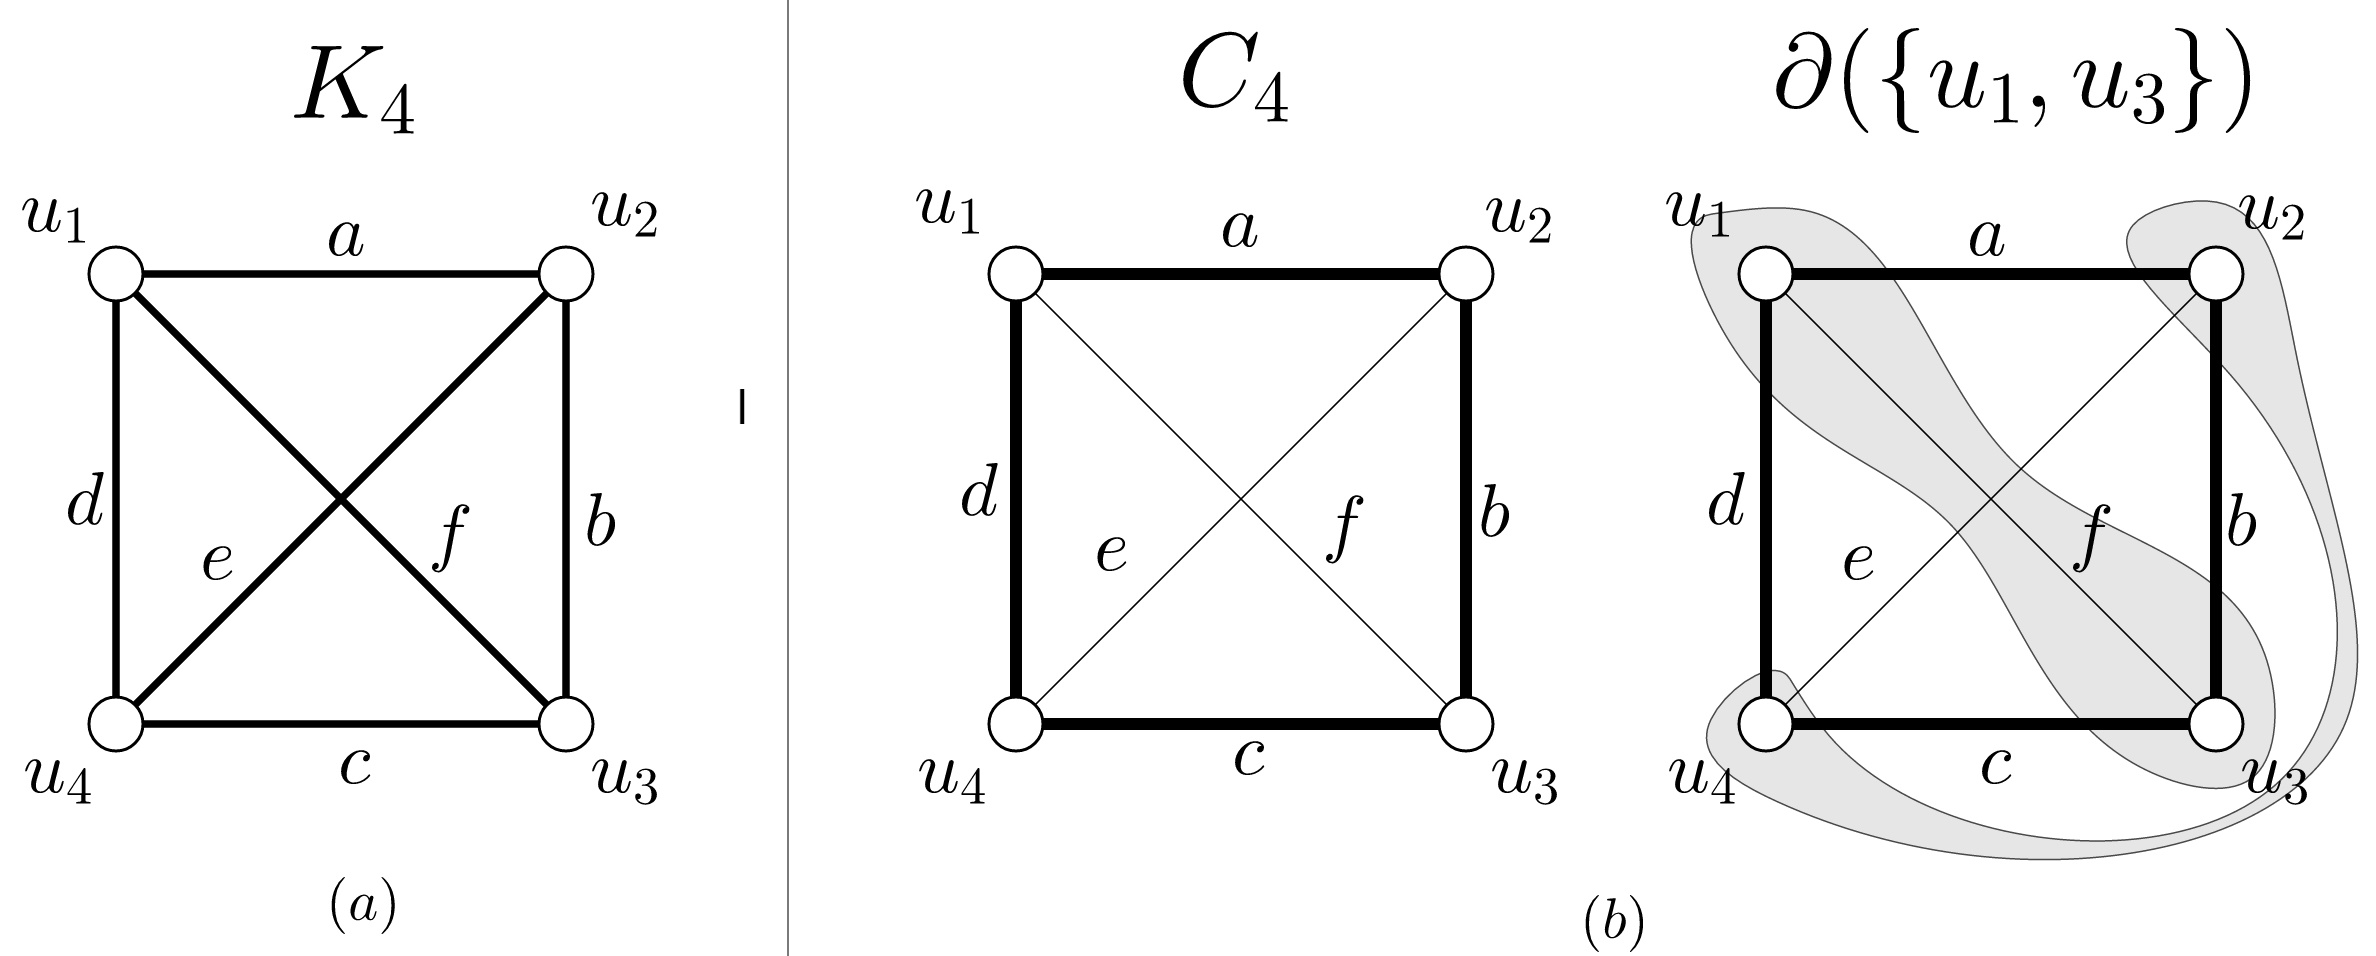
\includegraphics[scale=0.2]{img/imgchapter2/k4ciclocorte.jpg}
     \caption{}
     \label{fig:k4ciclocorte}
 \end{figure}

 \hfill $\blacklozenge$
\end{ejem}
 
 

 
 \section{Cortes y ciclos en digráficas}
 La teoría de digráficas tiene una amplia literatura, como puede verificarse en \cite{Bang-Jensen}. Sin embargo, en esta tesis realmente lo que nos interesa son las gráficas subyacentes de las digráficas. Concretamente, nos enfocaremos en sus cortes y sus gráficas pares y, desde luego, en los elementos minimales de estas clases de subgráficas. Por estas razones, sólo introducimos los conceptos necesarios para tal propósito.
 
 Las digráficas son de interés pues, como se verá en el próximo capítulo, permiten asociarles espacios vectoriales sobre los números reales (lo cual no sería posible si no tuvieran dirección los arcos).


 \subsection{Conjuntos de corte de $D$}
 Sean $X \subseteq V$ y $Y \subseteq V$. Al conjunto de arcos cuyas colas estén en $X$ y cabezas en $Y$ se le denota como $A[X,Y]$. Si $Y = \overline{X}$, $\partial^{+} (X) := A[X,\overline{X}]$ es el \textit{excorte}\index{Excorte de una digráfica} de $D$ asociado a $X$. Similarmente, el \textit{incorte} \index{Incorte de una digráfica}  asociado a $X$ es el conjunto $\partial^{-}(X) := A[X,\overline{X}]$. 
 
 Finalmente el \textit{conjunto de corte de $D$ asociado a $X$} \index{Conjunto de corte! de una digráfica} es la unión del excorte y el incorte respectivo, es decir, $\partial(X) := \partial^{+}(X) \cup \partial^{-}(X)$. Es sencillo observar que $\partial^{+}(X) = \partial^{-}(\overline{X})$. En la figura \ref{fig:excorteincorte} mostramos un excorte y un incorte de la digráfica del inciso $(a)$, con $X=\{u_{2},u_{3},u_{5}\}$.

 

Un uso de esta nueva notación es la de reescribir la definición de conexidad fuerte que dimos en un principio. En efecto, $D$ es \textit{fuertemente conexa} si y sólo si, para todo $X \subseteq V(D)$, $\partial^{+}(X) \neq \emptyset$. 

Asimismo, recordando la definición de la matriz de incidencia $\mathbf{M}_{D} = [m_{va}]$, podemos ahora establecer que:
\begin{equation} \label{eq:mva}
  m_{va}=
    \begin{cases}
\hspace{0.7em} 1, & a \in \partial^{+}(v)\\ 
-1, & a \in \partial^{-}(v)\\ 
\hspace{0.7em} 0, & \text{en otro caso}
\end{cases}
\end{equation}

 \begin{figure}[H]
    \centering
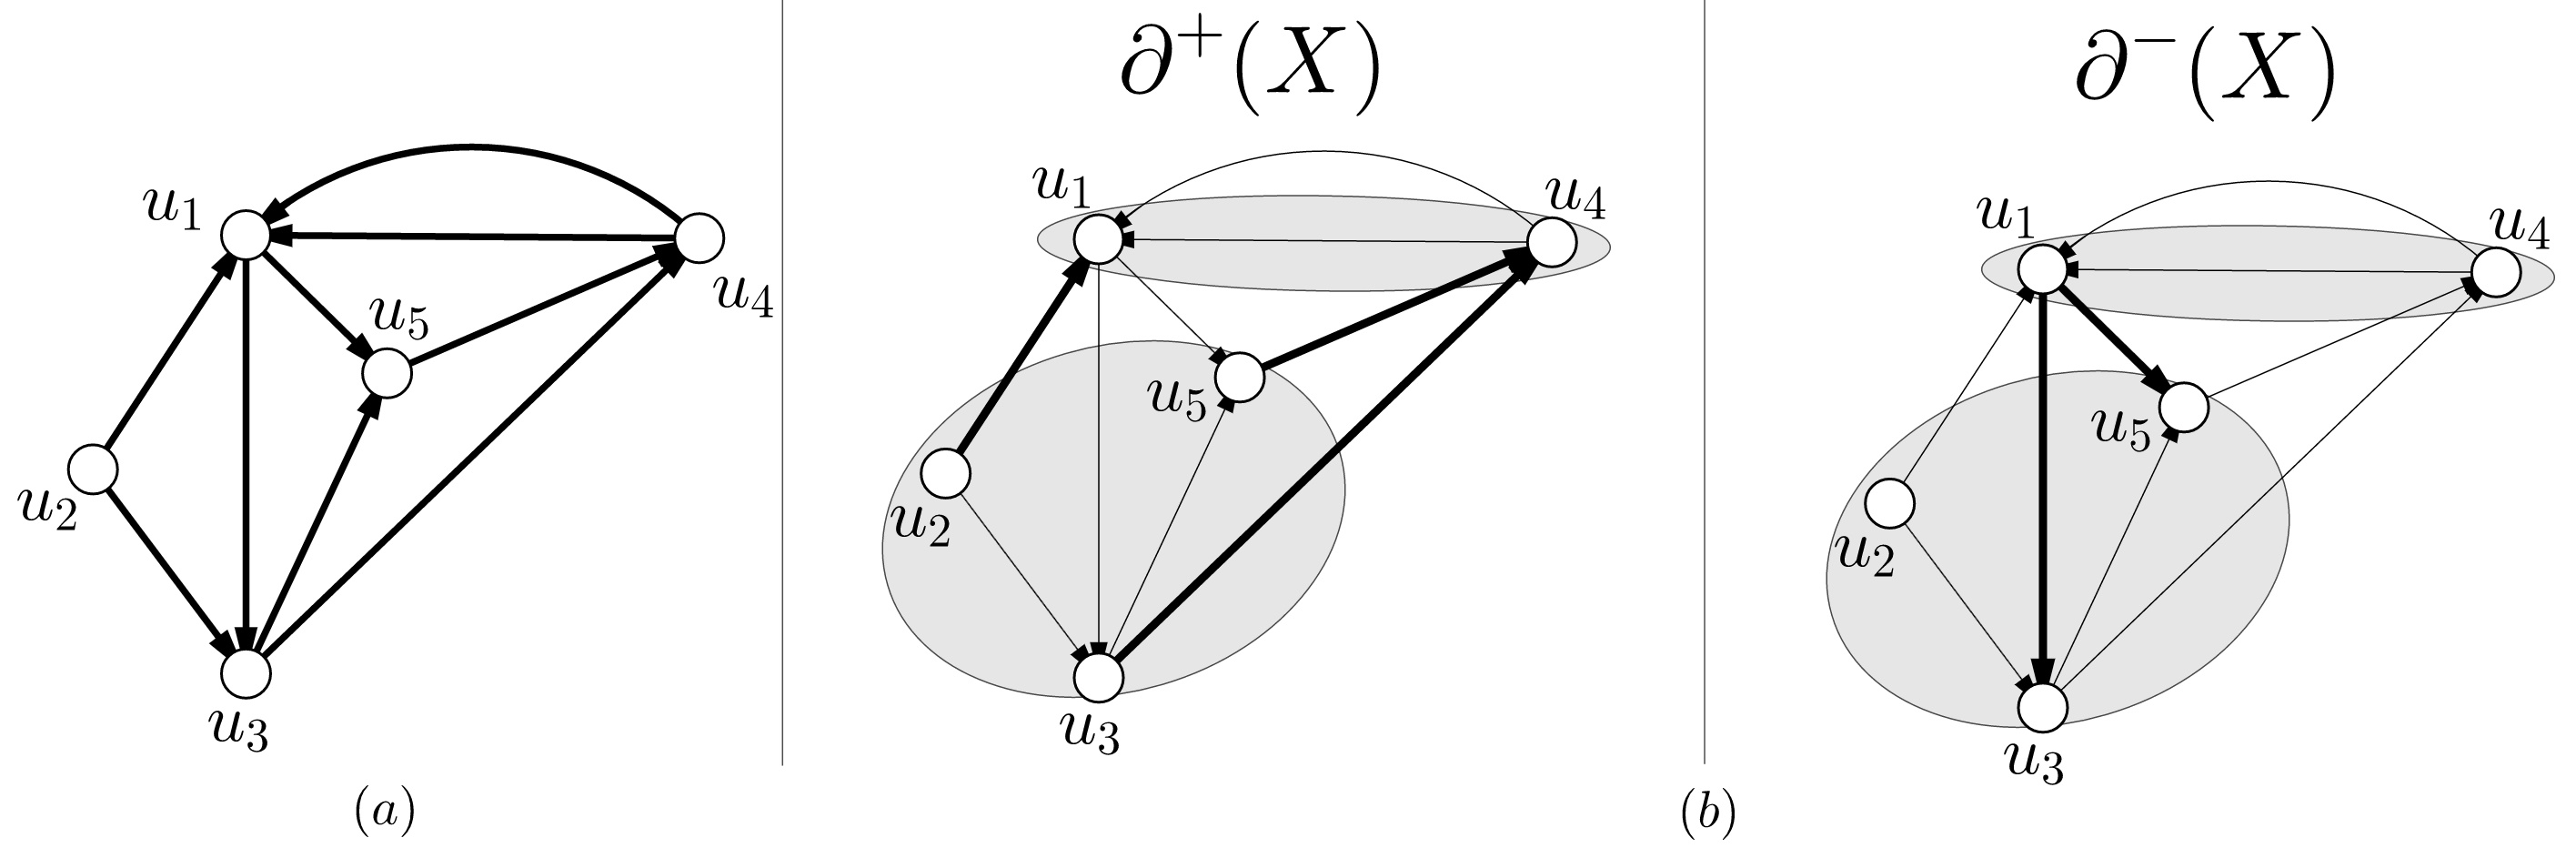
\includegraphics[scale=0.18]{img/imgchapter2/ExcorteIncorte.jpg}
    \caption{}
    \label{fig:excorteincorte}
\end{figure}

Si $G:=G(D)$ es la gráfica subyacente de $D$, observamos también que los elementos en $\partial_{G}(X)$ son los mismos que en $\partial_{D}(X)$ pero sin considerar direcciones. De aquí que un conjunto de aristas es un corte en $G$ si y sólo si el correspondiente conjunto de arcos es un corte en $D$.

Lo anterior nos abre paso para definir cortes minimales en digráficas. Así, un conjunto de corte $\partial_{D}(X)$ es \textit{minimal} \index{Conjunto de corte! minimal en una digráfica} en $D$ si y sólo si $\partial_{G}(X)$ es un corte minimal en $G$. También diremos que un conjunto de corte es \textit{dirigido} si $\partial(X) = \partial^{+}(X)$, o sea, $\partial^{-}(X)=\emptyset$.

Observemos que en cualquier corte dirigido, los cortes minimales que contiene también deben ser dirigidos. Apoyémonos de la figura \ref{fig:bondsdirigidos}. Si $\partial(X) = \partial^{+}(X)$, cualquier $\partial(Y) \subseteq \partial^{+}(X)$ es de la forma $\partial(Y) = A[X \cap Y, \overline{X} \cap \overline{Y}] \cup A[X \cap \overline{Y}, \overline{X} \cap Y] $. 

Por otro lado, si $B$ es un corte minimal contenido en $\partial(X)$, podemos tomar a $Y$ como el conjunto de colas de los arcos de $B$ (pensando en $B\subseteq A(D)$) y, por lo tanto, $\partial(Y) = B$. Lo anterior es posible porque los arcos de $B$ tiene una sola dirección (al ser elementos de $\partial(X)$). Sin embargo, por cómo se construyó $Y$, en realidad $Y\subseteq X$ y, en consecuencia, $\overline{X} \cap Y = \emptyset$-

Entonces $\partial(Y)= A[X \cap Y, \overline{X} \cap \overline{Y}] = \partial^{+}(Y)$. Por lo que \textit{todo corte minimal contenido en un corte dirigido debe ser, a su vez, dirigido}.

\begin{figure}[H]
    \centering
    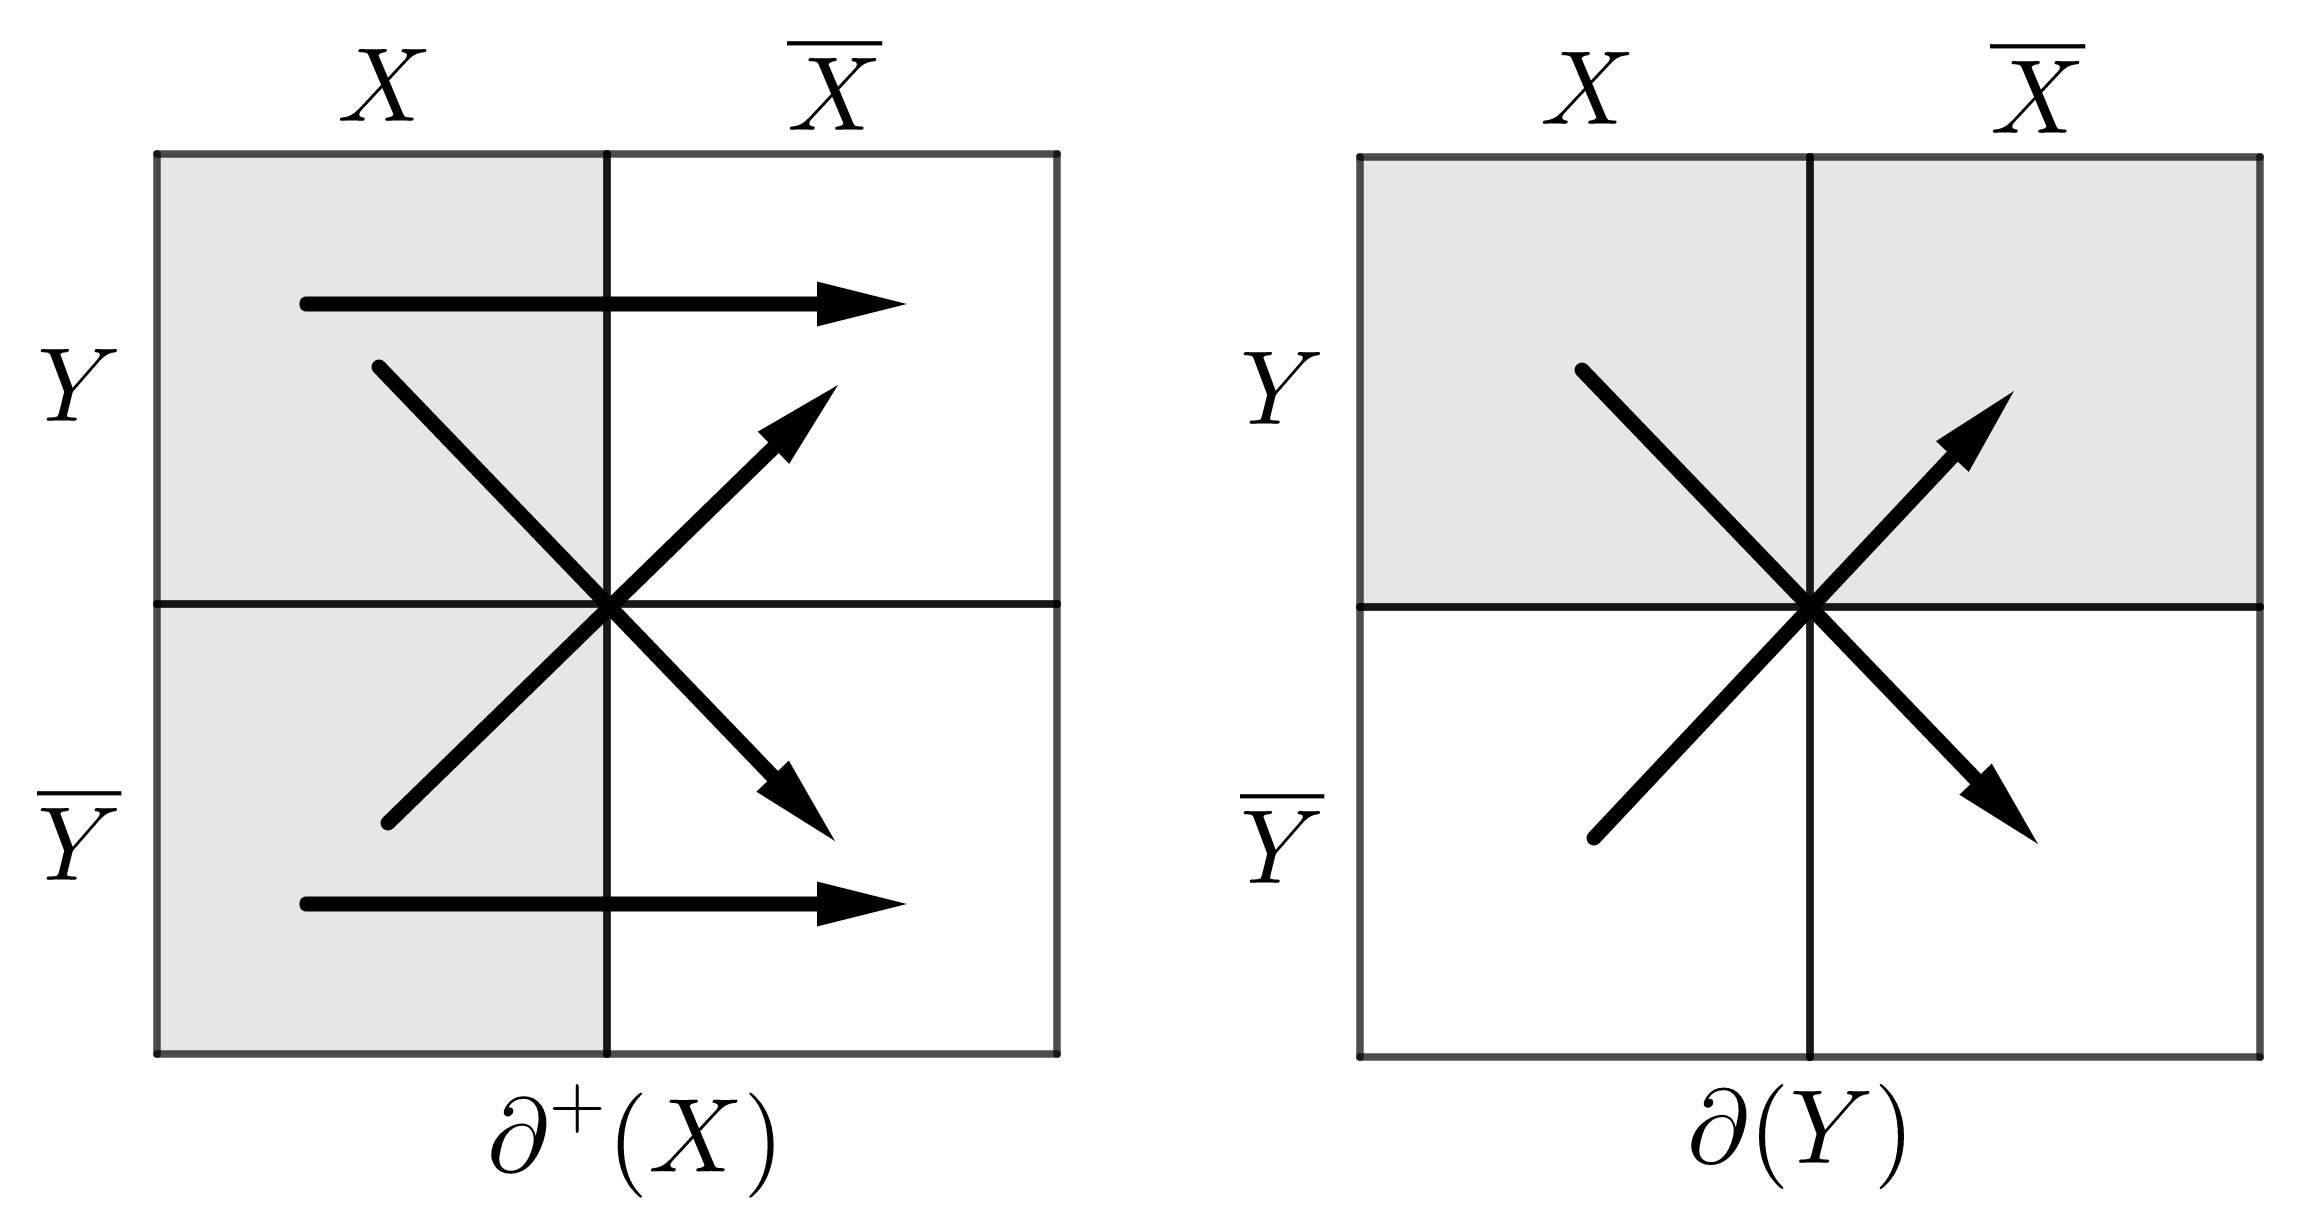
\includegraphics[scale=0.15]{img/imgchapter2/bondsdirigidos.jpg}
    \caption{}
    \label{fig:bondsdirigidos}
\end{figure}


 \subsection{Los ciclos de $D$}
 
Sea $C$ un ciclo de $D$, con vértices $V=\{u_{1}, \ldots, u_{n}\}$ y arcos $A=\{a_{1},\ldots, a_{n}\}$. Dependiendo del diagrama con el que representemos al ciclo, es sencillo convencerse que puede ser \textit{recorrido} (o \textit{atravesado}) en dos sentidos: a favor de las manecillas del reloj (representado con el símbolo $\mathbf{\circlearrowright}$) o en contra de las manecillas del reloj (cuyo símbolo asociado es $\mathbf{\circlearrowleft})$. Dicho formalment, podemos asociar a $C$ dos posibles circuitos distintos: $\Gamma_{\mathbf{\circlearrowright}}=u_{1}a_{1}u_{2}\ldots u_{n}a_{n}u_{1}$ y $\Gamma_{\mathbf{\circlearrowleft}}=u_{1}a_{n}u_{n}\ldots u_{2}a_{1}u_{1}$, suponiendo que los vértices y arcos han sido etiquetados \textit{en orden}.

\index{Arco! hacia adelante} \index{Arco! hacia atrás} No necesariamente $u_{i-1}$ domina a $u_{i}$ (en $\Gamma_{\mathbf{\circlearrowright}}$), ni tampoco siempre se cumple que  $u_{i}$ domina a $u_{i-1}$ (en $\Gamma_{\mathbf{\circlearrowleft}}$). Los arcos $a_{i}$ de $\Gamma_{\mathbf{\circlearrowright}}$ para los cuales sí se da que $t(a_{i}) = u_{i-1}$ y $h(a_{i})=u_{i}$ se llaman \textit{arcos hacia adelante} (\textit{Forward arcs}, en inglés); y aquellos tales que $t(a_{i})=u_{i}$ y $h(a_{i})=u_{i-1}$ son \textit{arcos hacia atrás} (\textit{Reverse arcs}, en inglés). Los arcos hacia adelante y atrás de $\Gamma_{\mathbf{\circlearrowleft}}$ son definidos análogamente.

Los conjunto de arcos hacia adelante y hacia atrás de $\Gamma_{\mathbf{\circlearrowright}}$ inducen dos subdigráficas del ciclo $C$, denotados, respectivamente, por $C^{+}_{\mathbf{\circlearrowright}}$ y $C^{-}_{\mathbf{\circlearrowright}}$. De manera similar, $\Gamma_{\mathbf{\circlearrowleft}}$ induce $C^{+}_{\mathbf{\circlearrowleft}}$ y $C^{-}_{\mathbf{\circlearrowleft}}$. Puede verificarse que $C^{+}_{\mathbf{\circlearrowright}}=C^{-}_{\mathbf{\circlearrowleft}}$ y $C^{-}_{\mathbf{\circlearrowright}} = C^{+}_{\mathbf{\circlearrowleft}} $

\begin{ejem}
En la imagen \ref{fig:ciclosentidos} mostramos un ciclo de nueve vértices y, para representar el sentido escogido, dentro de él colocamos el símbolo $\mathbf{\circlearrowright}$. Asimismo, resaltamos los arcos hacia adelante $C^{+}_{\mathbf{\circlearrowright}}$ y los arcos hacia atrás $C^{-}_{\mathbf{\circlearrowright}}$. 

\begin{figure}[H]
    \centering
    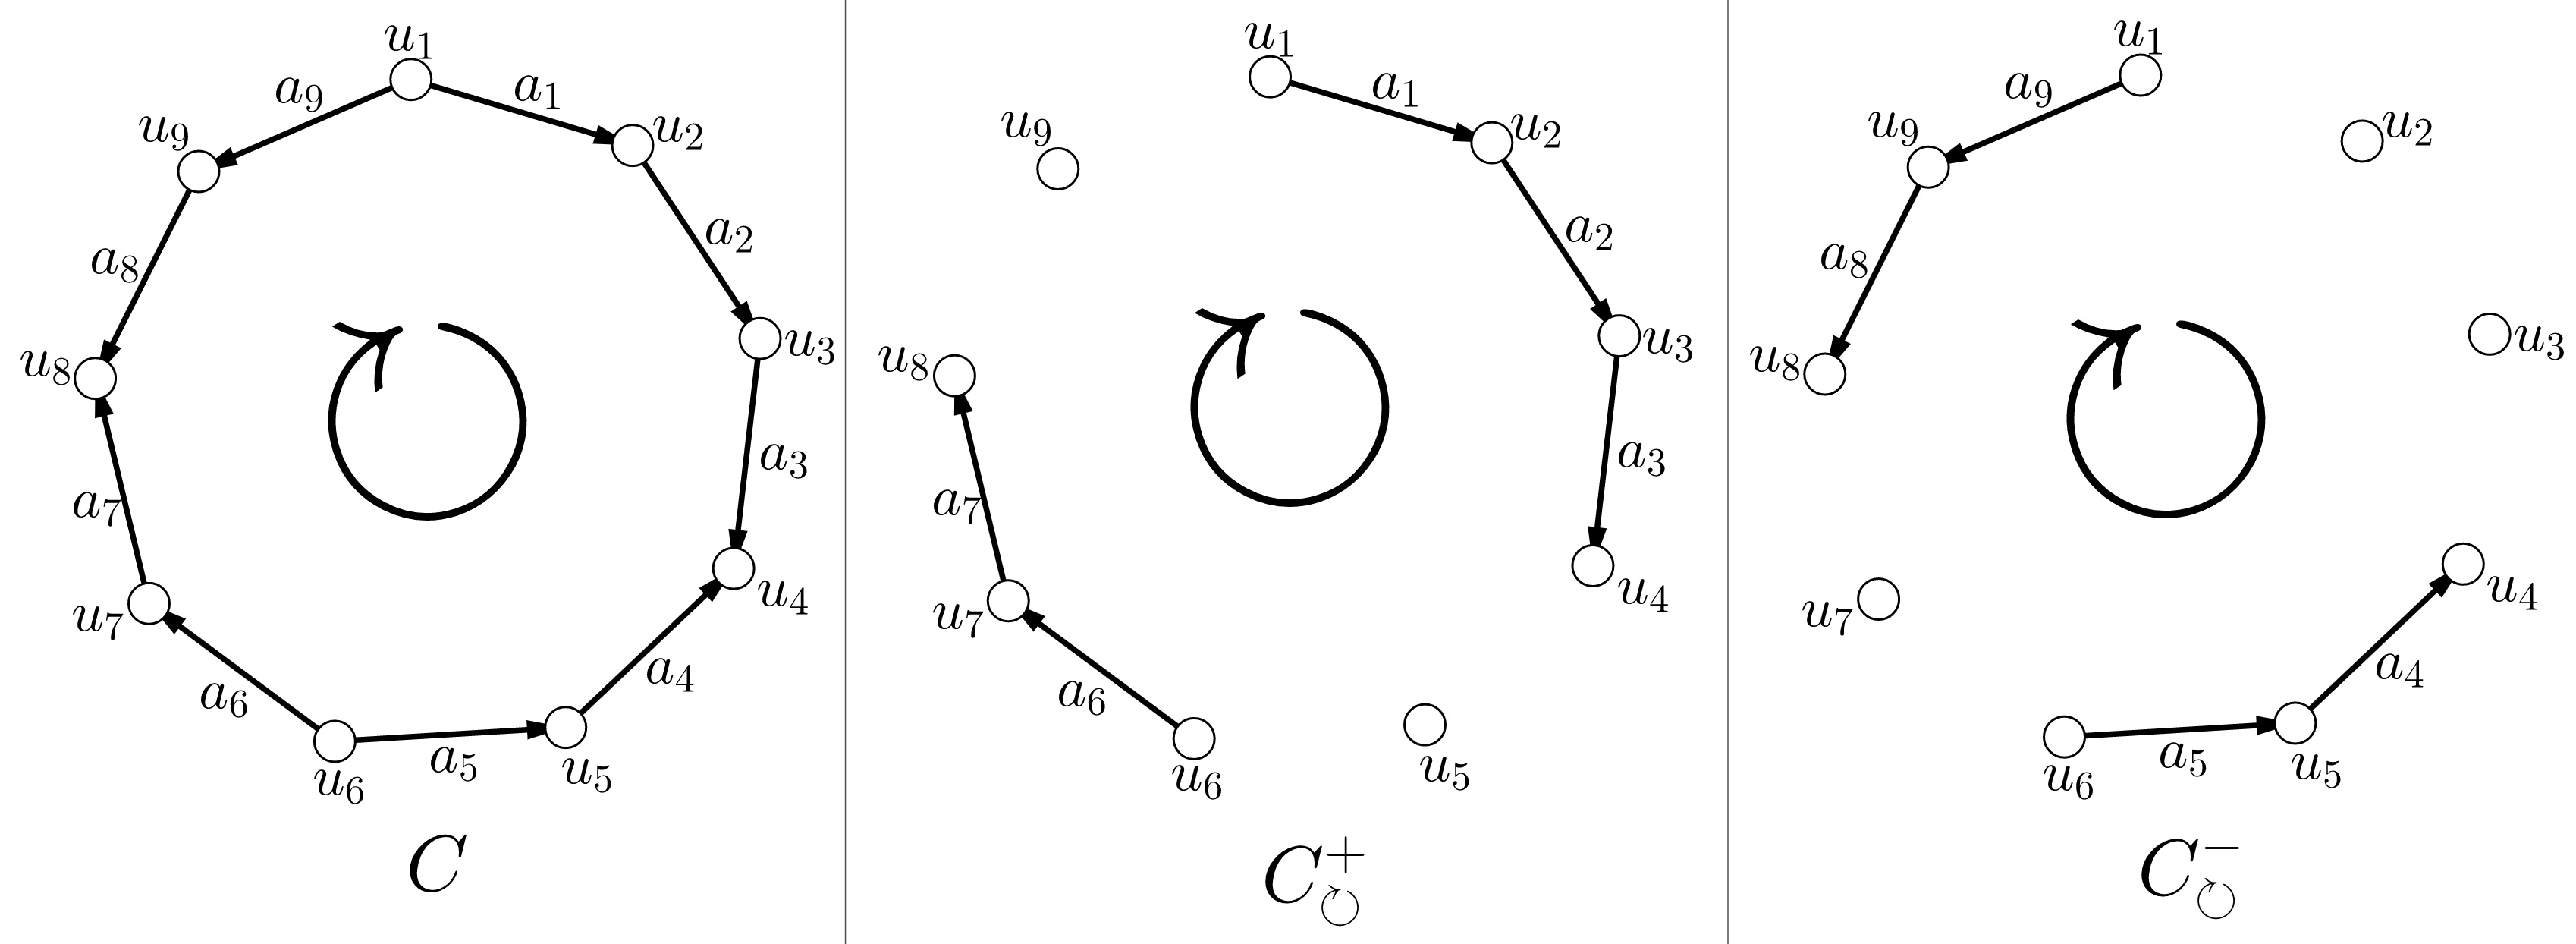
\includegraphics[scale=0.15]{img/imgchapter1/sentidociclos.jpg}
    \caption{}
    \label{fig:ciclosentidos}
\end{figure}

\hfill $\blacklozenge$
\end{ejem}

Sea cual sea el sentido que escojamos, es evidente que $C = C^{+} \cup C^{-}$. Aún más, si para algún sentido se tiene que $C=C^{+}$, entonces $C$ es un \textit{ciclo dirigido}. De hecho, se dice que una digráfica es \textit{Digráfica! acíclica}\textit{acíclica} si no contiene ciclos dirigidos. Por ejemplo, la digráfica de la figura \ref{fig:digrafoaciclico} es acíclica pues, aunque ella misma sea un ciclo, no es un ciclo dirigido. Una de sus propiedades más importantes que \textit{toda digráfica acíclica tiene, al menos, una fuente y un pozo.}


\begin{figure}[H]
 \centering
  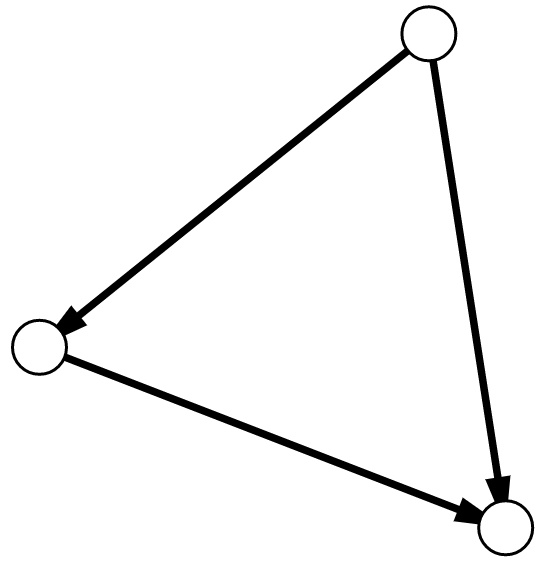
\includegraphics[scale=0.22]{img/imgchapter1/digrafoaciclico.jpg}
  \caption{}
  \label{fig:digrafoaciclico}
  %\vspace{-2 cm}
\end{figure}
